\documentclass[journal]{IEEEtran}

% --- Packages ---
\usepackage{amsmath,amssymb}
\usepackage{graphicx}
\graphicspath{{../results/figures/}{../forecasts/}}
\usepackage{booktabs}
\usepackage{siunitx}
\usepackage{url}
\usepackage[hidelinks]{hyperref}
\usepackage{cite}

% --- Title / Author ---
\title{Probabilistic Forecasting of ICE Coffee C Futures Returns via GARCH(1,1) with Student's $t$ Innovations}

\author{%
  Bridget~Brinkman,~Faith~Morrissey,~Yun-Chih~(Rick)~Wu,~Stella~McElwain,~and~Farah~Hendawy%
  \thanks{All authors are with the Department of Mathematics, University of Pittsburgh, Pittsburgh, PA 15260, USA.}%
  \thanks{Manuscript prepared in May 2026.}
}

\markboth{May 2026}{Brinkman \emph{et al.}: Probabilistic Forecasting of ICE Coffee C Futures}

\begin{document}
\maketitle

% =============================================================
\begin{abstract}
% =============================================================
This paper develops a probabilistic forecasting model for daily
ICE Coffee~C front-month futures, motivated by the procurement-planning
needs of a Pittsburgh-area specialty coffee roaster.  We proceed in two
parts.  Section~I constructs a 60-origin rolling-window backtest of ten
point-forecast models, ranging from a na\"ive drift baseline to the IBM
Granite Tiny Time Mixer foundation model.  Pairwise Diebold-Mariano tests
and a Model Confidence Set find that nine of the ten models are jointly
statistically indistinguishable from random-walk-with-drift at $\alpha=0.10$
on mean absolute error.  Section~II argues that this is not evidence of an
unstructured series but of an inappropriate forecasting target.  Coffee
returns exhibit pronounced volatility clustering and fat tails; these are
exploitable by density forecasts even when point forecasts cannot be
improved.  We fit a GARCH(1,1) model with standardized Student's $t$
innovations and evaluate its calibration on the same 60-origin walk-forward
backtest.  Empirical coverage of the model's prediction intervals tracks
nominal coverage within a few percentage points at every level evaluated,
and predictive-interval widths adapt smoothly to local volatility across
diverse historical regimes.
\end{abstract}

\begin{IEEEkeywords}
Time series, GARCH, density forecasting, volatility clustering, coffee
futures, probabilistic forecasting, interval calibration, Model Confidence Set.
\end{IEEEkeywords}

% =============================================================
\section{Rolling-Window Backtest of Point Forecasts}
% =============================================================
\label{sec:section1}

\subsection{Background and Motivation}
\label{sec:motivation_intro}

\IEEEPARstart{T}{his} project was motivated by the procurement-planning
needs of 19~Coffee~Company, a wholesale specialty coffee roaster based in
the South Hills of Pittsburgh, Pennsylvania.  19~Coffee sources beans
through direct-trade relationships with smallholder farms in regions
including Ethiopia, Colombia, Guatemala, Sumatra, and Kenya, and supplies
caf\'es, gourmet groceries, and restaurants across the Pittsburgh tri-state
area.  While 19~Coffee does not transact directly in the futures market,
the ICE Coffee~C contract is the global price benchmark to which their
input costs are ultimately tied through importer pricing and the
differential-to-C system (specialty contracts are priced as a fixed
premium above the C futures benchmark, so 19~Coffee's procurement costs
track C movements without direct market participation).  A
forecasting framework that produces calibrated uncertainty
intervals---rather than single-number point estimates---would inform
their procurement timing, contract negotiation, and budget planning.
Our objective across both sections of this paper is to develop and
validate such a framework.

\subsection{Data}
\label{sec:data_section1}

We use the daily front-month nearby continuous settlement series of ICE
Coffee~C futures, obtained from the ICE Report~293 historical price
service.\footnote{\url{https://www.ice.com/report/293}}  The series spans
January~1994 through January~2026 ($N = 8{,}104$ daily observations,
$8{,}103$ daily log returns after differencing).  Prices are quoted in
cents per pound (\textcent/lb).  Holiday closures and exchange suspensions
appear as gaps in the trading-day index but introduce no missing values in
the cleaned series.

\subsection{Forecasting Model Suite}
\label{sec:models_section1}

We select ten forecasting models spanning a deliberately wide range of
modeling paradigms---from na\"ive baselines through classical statistical
methods to recent foundation models---with the intent of testing whether
any class of model is able to extract structure that the others miss.  All models are evaluated through a uniform
\verb|predict(context_df, horizon)| interface so that the backtest runner
treats them as interchangeable.

\subsubsection{Na\"ive baselines (from \texttt{statsforecast}~\cite{statsforecast})}
\textbf{Na\"ive} repeats the last observed price for all horizons.
\textbf{RWD} (random walk with drift) repeats the last observed price plus
a linear drift equal to the mean training-window return.

\subsubsection{Classical statistical models (from \texttt{statsforecast})}
\textbf{Theta} decomposes the series into long-term trend and short-term
components.  \textbf{AutoETS} selects an exponential-smoothing
specification (error, trend, seasonality combinations) by information
criterion.  \textbf{AutoARIMA} selects an ARIMA$(p,d,q)$ specification
similarly.

\subsubsection{Recursive machine-learning models}
\textbf{Ridge} (linear regression with $\ell_2$ penalty) and
\textbf{Random Forest}~\cite{breiman2001} are fit on lag-based features
(lags $1, 2, 5, 10, 21, 63$) and rolling-window summaries (mean and
standard deviation over $5, 21, 63$ days), then iterated forward recursively
by feeding each prediction back as the next observation.

\subsubsection{Volatility model}
\textbf{GARCH} uses an AR(1) mean equation with GARCH(1,1) variance and
Gaussian innovations, fit on raw prices, with the point forecast taken
from the mean equation's $h$-step prediction.  We note that this is a
\emph{different} parameterization from the GARCH(1,1)+$t$ model used in
Section~II, where the mean equation is fixed at zero, the model is fit on
log returns, and the innovations are Student's~$t$.  The model in this
section is used as a point forecaster for direct comparison with other
point-forecast methods; Section~II uses GARCH as a density forecaster.

\subsubsection{Decomposition model}
\textbf{Prophet}~\cite{taylorletham2018} with yearly seasonality and no
daily seasonality.

\subsubsection{Foundation model (zero-shot)}
\textbf{Granite~TTM}~\cite{eknathekar2024ttm} is the IBM Granite Tiny Time
Mixer~R2, a transformer-based foundation model for time-series forecasting
pretrained on a large multi-domain corpus.  We use the zero-shot variant
with a 1\,536-step context window; the context is per-window
standard-scaled before inference and de-scaled after.  Granite's context
length requirement is what motivates the 1\,536-day training window used
uniformly across all models in this backtest.

\subsection{Backtest Design}
\label{sec:backtest_design}

We use a fixed-length rolling-window backtest.  At each forecast origin
$T_k$, models are fit on the prior 1\,536~trading days
$\{P_{T_k - 1535}, \dots, P_{T_k}\}$ and forecast 63~trading days ahead
(approximately one calendar quarter).  Forecast accuracy is evaluated against
the realized prices $\{P_{T_k+1}, \dots, P_{T_k+63}\}$.

\textbf{Choice of number of origins.}  The number of origins evolved
during the project.  At one origin (the most recent 63~days of data),
Granite-TTM produced the lowest mean absolute error
(20.88\,\textcent/lb versus RWD's 29.23, a 28\,\% gap), consistent with our
initial expectation that mechanistic complexity would correlate with
forecast accuracy.  Fig.~\ref{fig:holdout} shows all ten models'
forecasts at this single origin; most predict a flat-to-upward path
while the realized price declined sharply, and even the three models
that trended downward (Granite-TTM, RF, GARCH) substantially
underestimated the magnitude of the decline.  We then scaled to
10, 30, and finally 60 evenly-spaced origins, with the spacing fixed at
110~days such that consecutive forecast horizons do not overlap.  At
60~origins, the design covers approximately 80\,\% of the full series
($\sim$2000 through 2025).  Fig.~\ref{fig:origins} visualizes the four
origin configurations on the price timeline.  The rankings at
60~origins, reported below, \emph{invert} the single-origin verdict:
Granite-TTM falls to eighth (MAE 13.84) and RWD becomes the leader
(MAE 12.79).

\begin{figure*}[t]
\centering
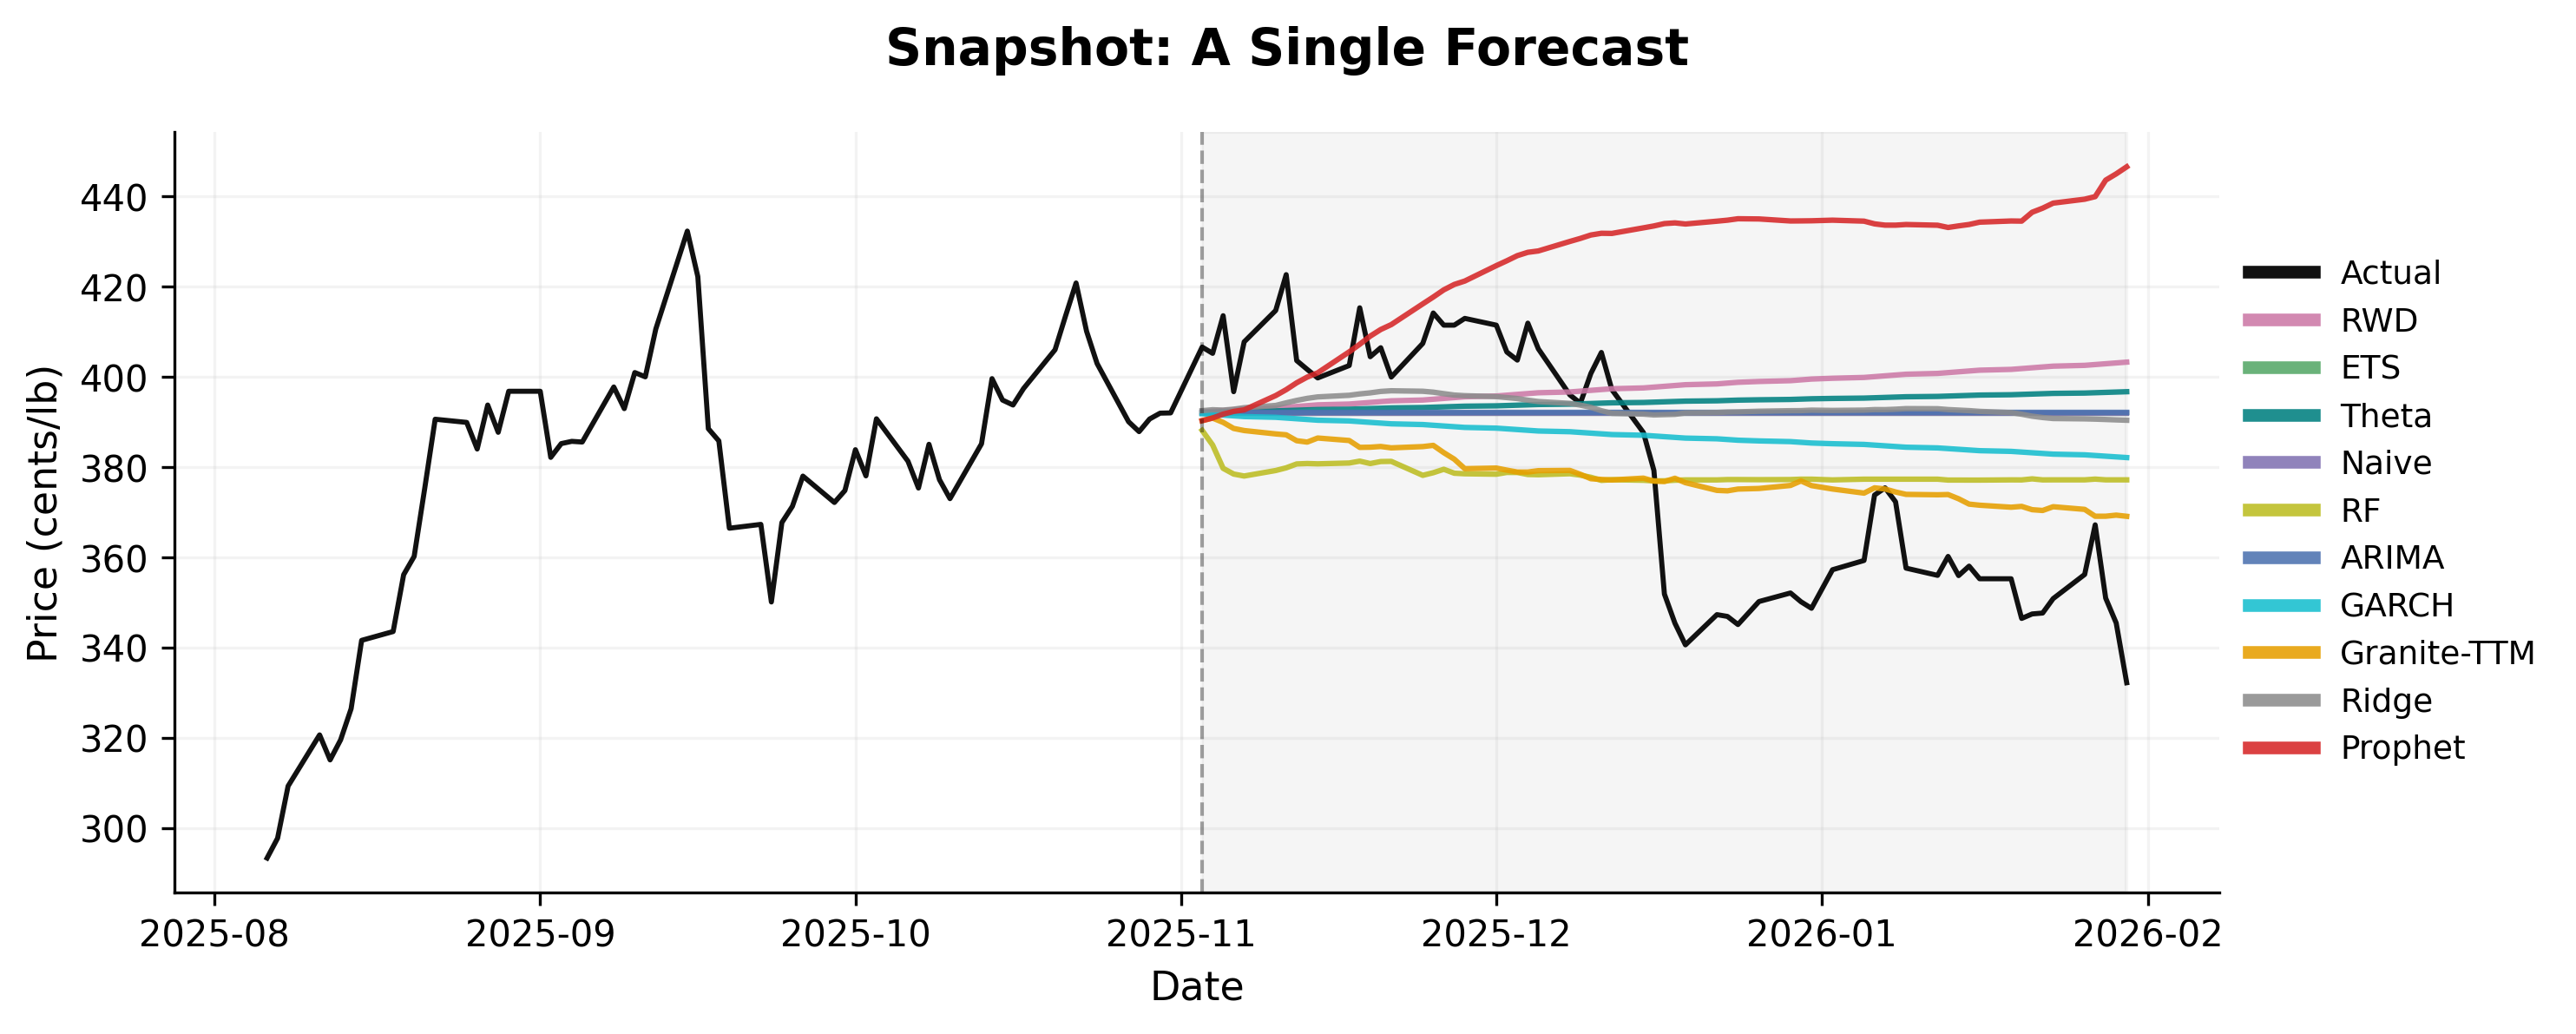
\includegraphics[width=0.85\textwidth]{coffee_holdout_plot.png}
\caption{Forecasts from all ten models at the single most recent
forecast origin (November~2025).  The dashed vertical line marks the
origin; historical prices appear to its left and 63-day forecasts from
all ten models to its right.  The actual price declined from
approximately 400 to 330\,\textcent/lb over the horizon.  Naive, ETS,
and ARIMA produce nearly identical flat-line forecasts at this origin
and overlap heavily in the plot.}
\label{fig:holdout}
\end{figure*}

\begin{figure*}[t]
\centering
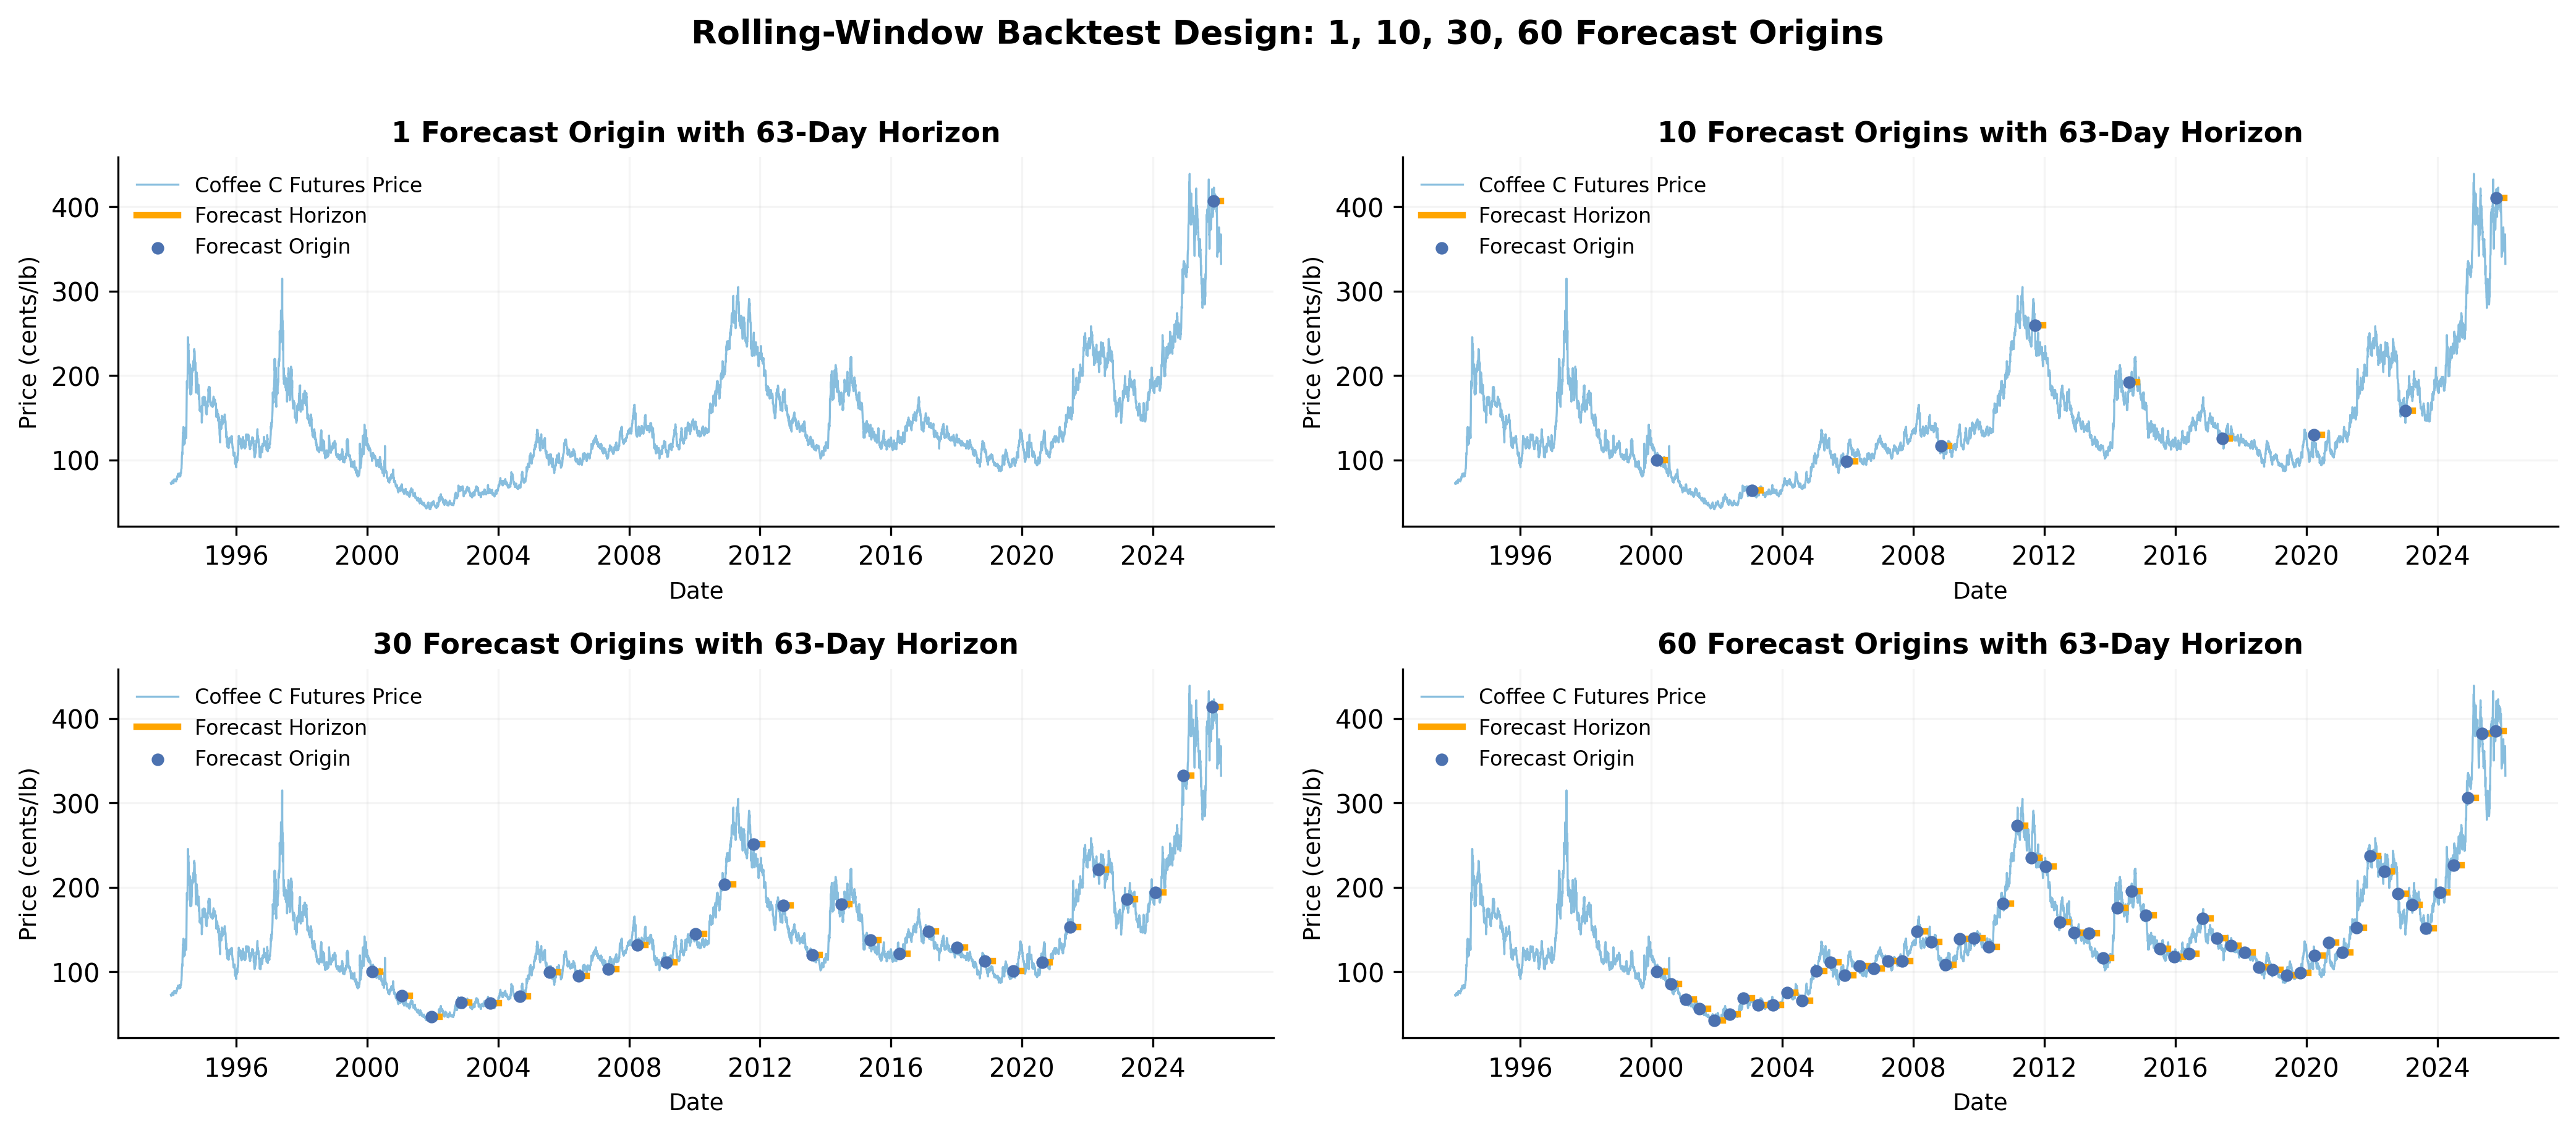
\includegraphics[width=0.95\textwidth]{forecast_origin_coverage.png}
\caption{Rolling-window backtest design at four scales: 1, 10, 30, and
60 forecast origins.  Each blue dot marks a forecast origin; each orange
segment shows the 63-day forecast horizon evaluated against realized
prices.  The single-origin design (top left) places its only test at the
end of the series, during the 2024--2025 rally---conditions that, by
chance, favor mechanically complex models.  The 60-origin design
(bottom right) covers approximately 80\,\% of the available series and
samples many regimes; this is the design under which the leaderboard in
Table~\ref{tab:leaderboard} is computed.}
\label{fig:origins}
\end{figure*}

\textbf{Evaluation metrics.}  We report mean absolute error~(MAE) as the
primary metric, with root mean squared error (RMSE) and symmetric mean
absolute percentage error (sMAPE) reported as supporting metrics.

\subsection{Leaderboard}
\label{sec:results_section1}

Table~\ref{tab:leaderboard} reports mean error metrics across all
60~forecast origins, sorted ascending by MAE.

\begin{table}[t]
\caption{Point-forecast leaderboard at 60~rolling forecast origins, sorted
ascending by mean MAE (cents/lb).}
\label{tab:leaderboard}
\centering
\small
\begin{tabular}{lccc}
\toprule
Model & MAE & RMSE & sMAPE \\
\midrule
RWD         & 12.79 & 14.84 & 0.083 \\
ETS         & 12.82 & 14.89 & 0.085 \\
Theta       & 12.86 & 14.93 & 0.085 \\
Na\"ive     & 12.91 & 14.99 & 0.085 \\
RF          & 13.13 & 15.19 & 0.087 \\
ARIMA       & 13.24 & 15.39 & 0.085 \\
GARCH       & 13.50 & 15.74 & 0.090 \\
Granite-TTM & 13.84 & 16.09 & 0.092 \\
Ridge       & 14.68 & 17.16 & 0.101 \\
Prophet     & 22.69 & 24.99 & 0.152 \\
\bottomrule
\end{tabular}
\end{table}

Three features of the leaderboard warrant comment.  First, RWD produces
the lowest mean MAE despite being one of the simplest models in the suite.
Second, the top four models (RWD, ETS, Theta, Na\"ive) sit within
0.12\,\textcent/lb of each other---a gap small enough to fall well within
any reasonable margin of sampling noise.  Third, Granite-TTM, the
foundation model whose pretraining was the source of our initial
optimism, places eighth out of ten and is outperformed by every classical
statistical baseline.  Prophet sits well outside the cluster of nine and
forms the only large absolute gap on the leaderboard.

\subsection{Statistical Tests: Diebold-Mariano and the Model Confidence Set}
\label{sec:dm_mcs}

The leaderboard is descriptive but does not resolve statistical
significance.  We apply two complementary tools.

\subsubsection{Diebold-Mariano test}
Each model is compared pairwise to the RWD baseline using the
Diebold-Mariano test~\cite{dieboldmariano1995}, with the
Harvey-Leybourne-Newbold small-sample correction~\cite{harveyleybournenewbold1997}.
The loss series is per-origin MAE (60~values per model), and the long-run
variance is estimated with a Newey-West HAC
estimator~\cite{neweywest1994} using the Bartlett kernel and the rule-of-thumb
bandwidth $\lfloor 4(T/100)^{2/9} \rfloor$.

\subsubsection{Model Confidence Set}
We apply the Model Confidence Set (MCS) of Hansen, Lunde, and
Nason~\cite{hansenlundenason2011} to identify the set of models
\emph{jointly} indistinguishable from the best, at significance level
$\alpha=0.10$.  Null distributions are obtained by circular block
bootstrap with block size~5 and $B = 5{,}000$ replicates.

\subsubsection{Results}
Fig.~\ref{fig:dm_mcs} summarizes both tests.

\begin{figure*}[t]
\centering
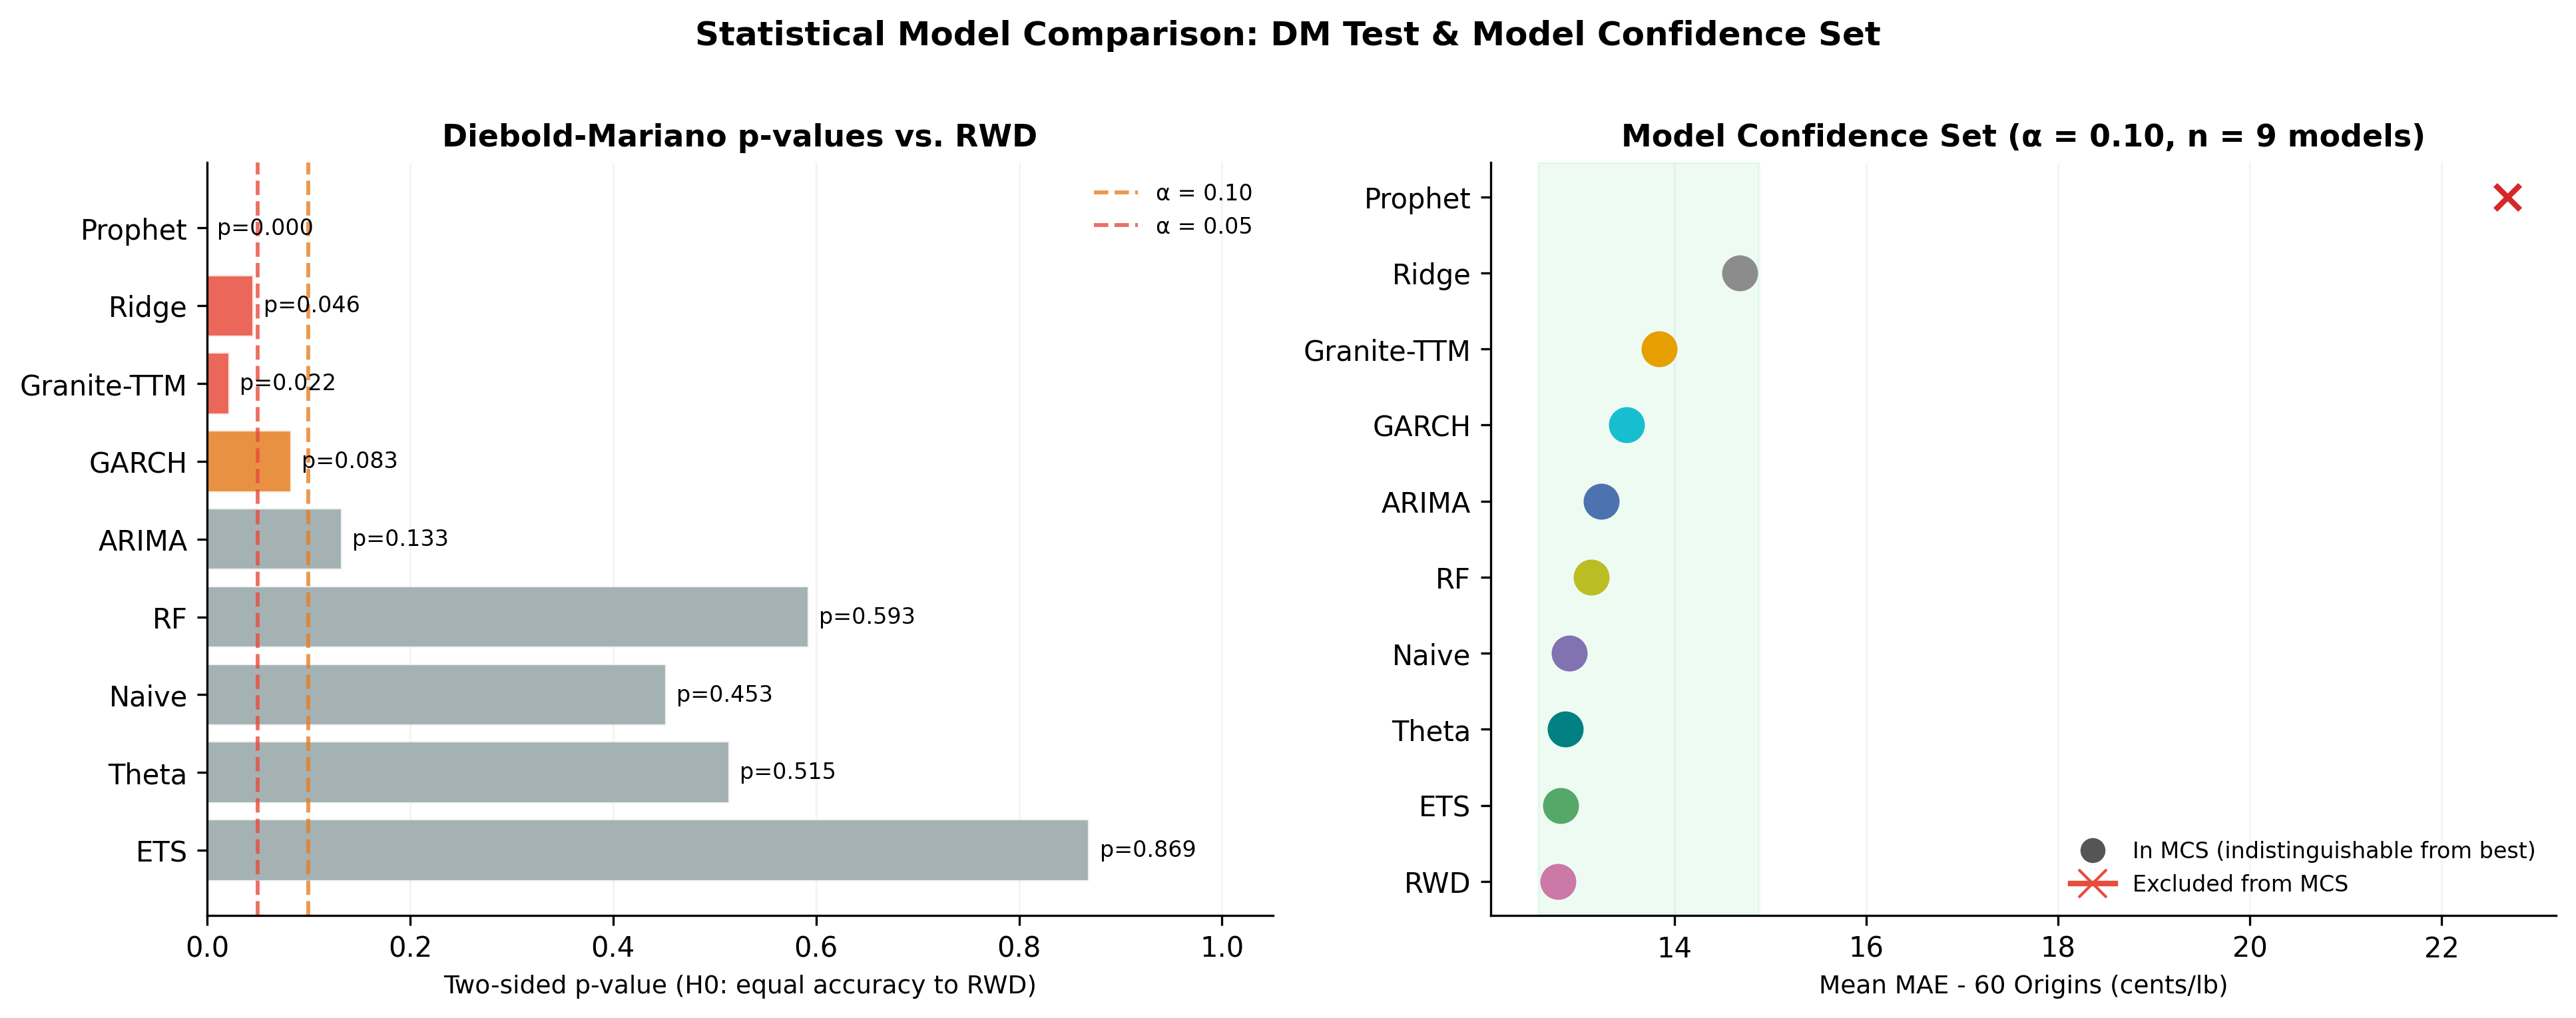
\includegraphics[width=0.85\textwidth]{dm_mcs.png}
\caption{Statistical comparison of the ten point-forecast models at 60~origins.
(a)~Pairwise Diebold-Mariano $p$-values testing each model against RWD;
bars are colored red for significance at $\alpha=0.05$ and orange at
$\alpha=0.10$. (b)~Model Confidence Set membership at $\alpha=0.10$; filled
dots are retained, the red cross is excluded.  Nine of ten models---all
except Prophet---are jointly indistinguishable from the best.}
\label{fig:dm_mcs}
\end{figure*}

The pairwise DM test rejects the equal-accuracy null at $\alpha=0.05$ for
Granite-TTM ($p = 0.022$), Ridge ($p = 0.046$), and Prophet
($p < 0.001$), and marginally for GARCH ($p = 0.083$).  All four
top-tier simple models (ETS, Theta, Na\"ive, RF) have $p > 0.4$ against RWD.

The MCS at $\alpha = 0.10$ retains nine of the ten models, eliminating only
Prophet (MCS $p = 0.009$).  The retained set spans every category in the
model suite: na\"ive baselines, classical statistical models, recursive
ML models, the volatility model, and the foundation model.

The MCS result is the appropriate primary inference because it
incorporates the multiple-comparisons correction implicit in evaluating
ten models against a single baseline.  The pairwise DM rejections of
Granite-TTM and Ridge do not survive joint correction; with ten
candidates being compared, the family-wise Type~I rate inflates well
above the nominal $\alpha$ of any single test.  We note also that
$T = 60$~origins is small relative to the simulation regimes in which
the MCS test is typically calibrated~($T \geq 100$), so the wide MCS
partly reflects limited test power; further origins would likely shrink
the surviving set, but the qualitative conclusion---no mechanism in this
suite reliably beats RWD---is robust.

\subsection{Section~I Conclusion: The Random-Walk Boundary}
\label{sec:section1_conclusion}

A diverse ten-model suite, ranging from na\"ive baselines to a
foundation model with cross-domain pretraining, cannot be statistically
distinguished from the random-walk-with-drift forecaster on the coffee
front-month series at 60~origins.  This pattern admits a natural
interpretation in financial economics: it is consistent with weak-form
market efficiency~\cite{fama1970}, the hypothesis that past prices alone
contain no exploitable information about future prices, and is the
empirical fingerprint one would expect on a price series whose direction
is essentially unpredictable from its own history.

This finding could be read narrowly as ``no~model helps,'' but that
reading would mistake the scope of the test.  Section~I evaluates
\emph{point} forecasts under \emph{absolute-error} loss.  Coffee returns
contain substantial structure beyond their mean---in particular,
time-varying volatility and fat tails---that point-forecast MAE is
constitutionally incapable of rewarding.  Section~II reframes the
forecasting target to expose this structure.

% =============================================================
\section{Probabilistic Forecasting via GARCH(1,1)}
% =============================================================
\label{sec:section2}

\subsection{From Point to Density Forecasts}
\label{sec:motivation}

A point forecast collapses a predictive distribution into a single number,
typically its mean or median.  For a series whose direction is approximately
unpredictable on short horizons, the best point forecast of tomorrow's price
is essentially today's price, and the best point forecast over a horizon $h$
is the current price (or current price compounded by a tiny drift).  This
is what Section~I observed: across ten candidate models, no method
materially outperformed RWD on MAE.

Point-forecast MAE, however, ignores the spread of the predictive
distribution.  A point forecast tells a procurement manager what the
``expected'' price is; a density forecast tells them what range of prices
is plausible.  An interval forecast can be used to size positions, price
options, set risk limits, or trigger contingent decisions, in ways that a
point forecast cannot.  This is the forecast object 19~Coffee would
actually use---an interval rather than a point---and it is the object
Section~II constructs.

The structure that motivates this richer forecasting target is well
known in the empirical finance literature \cite{mandelbrot1963,cont2001,tsay2010}
and is clearly visible in the coffee series.  We summarize the relevant
\emph{stylized facts} below.

\subsection{Data and Stylized Facts}
\label{sec:data}

Throughout, $P_t$ denotes the daily settlement price (cents per pound) at
trading day~$t$, and $r_t = \log(P_t / P_{t-1})$ denotes the daily log
return.  Log returns are preferred over simple returns because they are
additive across time: the $h$-day log return is the sum of $h$~consecutive
daily log returns.

Fig.~\ref{fig:prices_returns} displays $P_t$ together with $r_t$.  Three
features are immediately apparent.  First, prices wander without a stable
mean, ranging over more than an order of magnitude---from roughly
42\,\textcent\,/lb during the 2001--2002 bear market to a peak above
430\,\textcent\,/lb during the 2024--2025 rally.  Second, the magnitude of
daily returns varies substantially over time: the periods 1994--2000,
2011--2014, and 2024--2025 contain visibly larger moves than the calmer
stretches in 2005--2010 and 2017--2020.  Third, even within turbulent
regions, the \emph{sign} of returns shows no obvious pattern.

\begin{figure}[t]
\centering
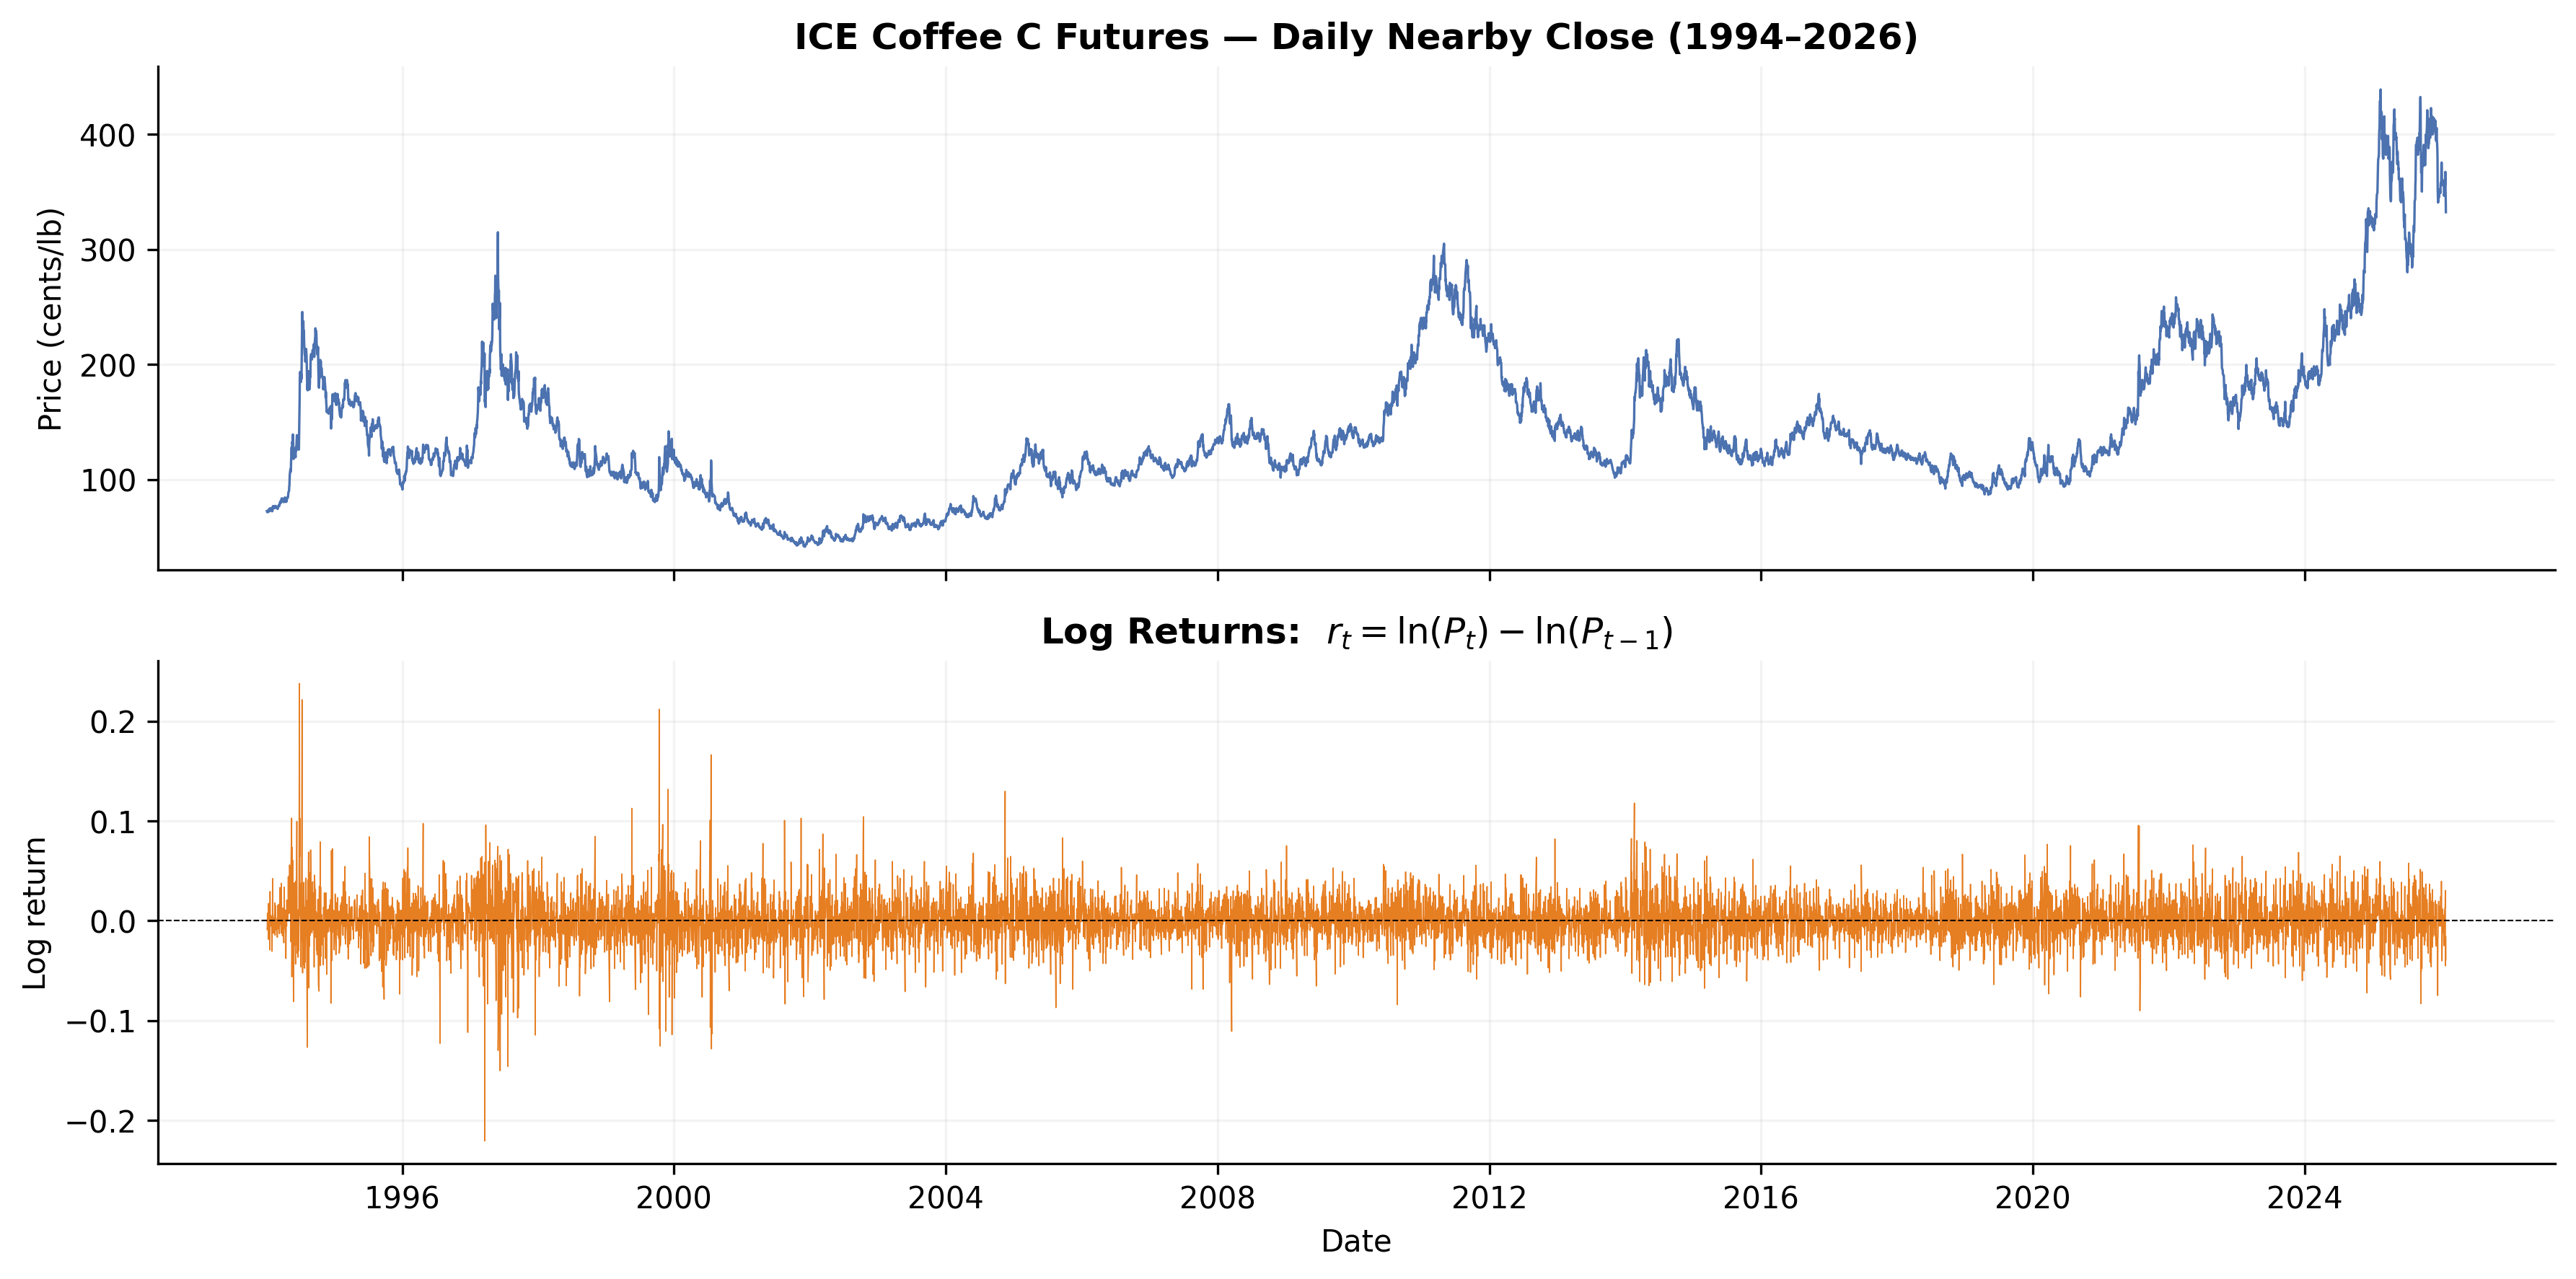
\includegraphics[width=\linewidth]{prices_vs_logreturns.png}
\caption{ICE Coffee C nearby front-month futures.  (a)~Daily settlement
price, January 1994 through January 2026.  (b)~Corresponding daily log
returns.  Note the visibly higher amplitude of returns during 1994--2000
and 2024--2025 compared to 2005--2010 or 2017--2020.}
\label{fig:prices_returns}
\end{figure}

These observations correspond to three quantifiable stylized facts.

\subsubsection{Stationarity}
An Augmented Dickey-Fuller test~\cite{dickeyfuller1979} on $P_t$ fails to
reject the unit-root null hypothesis ($p \approx 0.56$), confirming that
prices are non-stationary.  The same test applied to $r_t$ rejects the null
overwhelmingly ($p < 10^{-30}$).  Returns are therefore the natural object
of analysis.

\subsubsection{Fat-tailed return distribution}
Daily returns have sample mean $\hat{\mu} = 1.88 \times 10^{-4}$
(approximately $4.7\,\%$ annualized at $\hat\mu \cdot 252$), sample standard
deviation $\hat{\sigma} = 0.0237$ (approximately $37.6\,\%$ annualized at
$\hat{\sigma} \sqrt{252}$), sample skewness $0.19$, and \emph{excess}
kurtosis $6.65$.  The excess kurtosis is roughly an order of magnitude
larger than would be expected from a Gaussian process; consistent with this,
the daily series contains 31~moves of magnitude exceeding $10\,\%$, where a
Gaussian distribution calibrated to the sample variance would predict
essentially zero such moves over the same sample size.

Fig.~\ref{fig:distribution}(a)~plots the empirical density against
maximum-likelihood Gaussian and Student's~$t$ fits, and
Fig.~\ref{fig:distribution}(b)~shows the corresponding Normal Q-Q plot.
Both ends of the Q-Q plot curve sharply away from the diagonal, the
signature of tails fatter than the Gaussian benchmark; the Student's~$t$
density captures both the high central peak and the heavy tails that the
Gaussian cannot accommodate.

\begin{figure}[t]
\centering
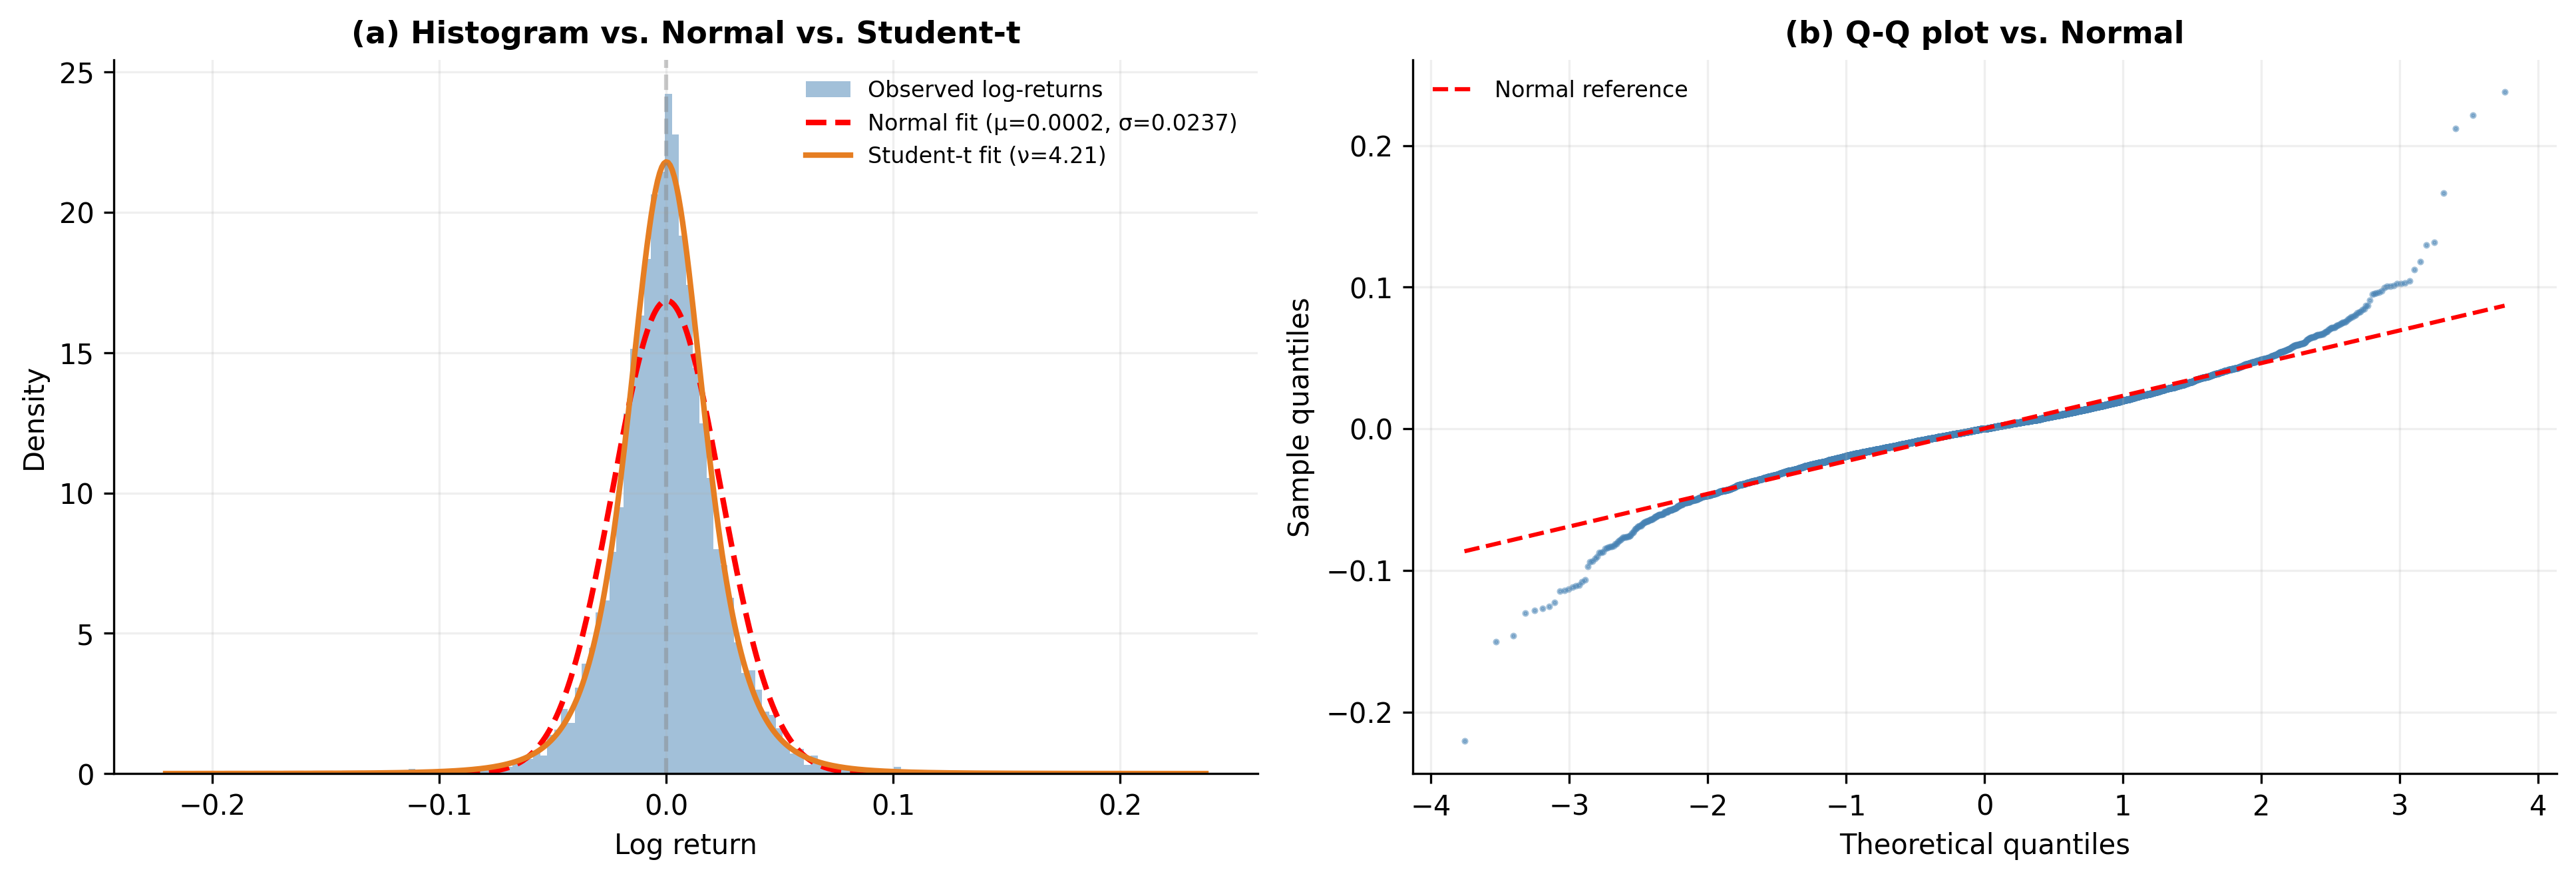
\includegraphics[width=\linewidth]{returns_distribution.png}
\caption{Distributional diagnostics for daily log returns. (a)~Empirical
density (bars) versus fitted Gaussian (dashed) and Student's~$t$ (solid)
densities.  The Student's~$t$ density captures both the high central
peak and the heavy tails; the Gaussian fits neither.  (b)~Normal Q-Q
plot.  Sharp departures from the diagonal at both ends confirm tails
fatter than Gaussian.}
\label{fig:distribution}
\end{figure}

\subsubsection{Volatility clustering}
Fig.~\ref{fig:acf} plots the empirical autocorrelation function~(ACF) of
returns $r_t$ and of their squared values $r_t^2$ at lags $1, \dots, 40$.
The two panels are visually distinct.  The ACF of $r_t$
[Fig.~\ref{fig:acf}(a)] sits essentially within the 95\,\% confidence band
at all lags, consistent with returns themselves being approximately
uncorrelated and consistent with Section~I's finding that no point-forecast
model could beat RWD.  The ACF of $r_t^2$ [Fig.~\ref{fig:acf}(b)] is large
at lag~1 ($\approx 0.14$) and decays slowly, remaining well above the
confidence band for at least 40~lags.

\begin{figure}[t]
\centering
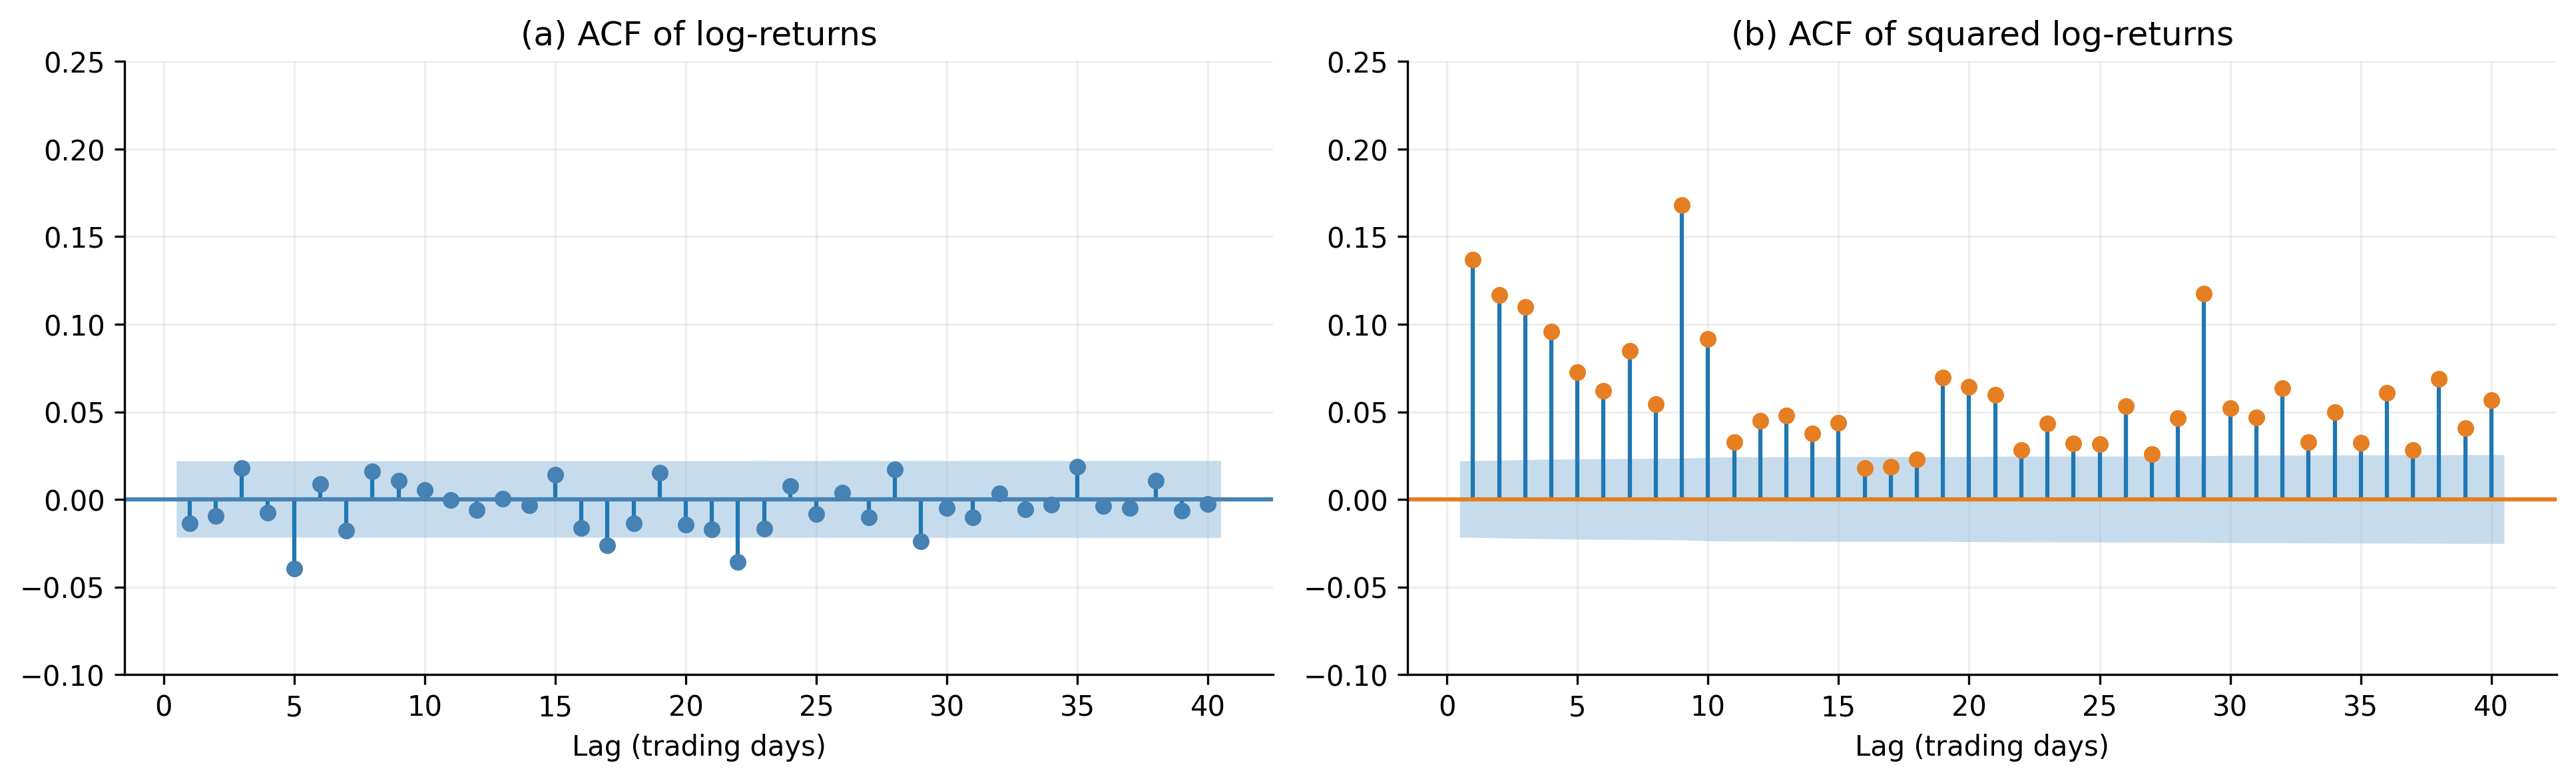
\includegraphics[width=\linewidth]{acf_returns_vs_squared.png}
\caption{Autocorrelation functions of (a)~daily log returns $r_t$ and
(b)~squared returns $r_t^2$, lags 1 through 40.  Shaded regions are
95\,\% confidence bands under the null of zero autocorrelation.  The
contrast between the two panels is the empirical signature of volatility
clustering.  A Ljung-Box test~\cite{ljungbox1978} of zero autocorrelation
through lag~20 yields $p \approx 0.006$ for $r_t$ and $p < 10^{-200}$ for
$r_t^2$.}
\label{fig:acf}
\end{figure}

This contrast---near-zero autocorrelation in returns but strong,
persistent autocorrelation in their magnitudes---is the empirical content of
\emph{volatility clustering}.  It implies that while the next return's
direction is essentially unforecastable, its expected \emph{magnitude} can
be predicted from recent magnitudes.  Modeling this structure is the
purpose of the GARCH framework.

\subsection{Model Specification}
\label{sec:model}

Following~\cite{bollerslev1986,bollerslev1987}, we specify the daily
return process as
\begin{equation}
\label{eq:garch_main}
r_t = \sigma_t z_t,
\quad z_t \overset{\text{i.i.d.}}{\sim} t^{*}_\nu,
\end{equation}
\begin{equation}
\label{eq:garch_var}
\sigma_t^2 = \omega + \alpha\, r_{t-1}^2 + \beta\, \sigma_{t-1}^2,
\end{equation}
where $t^{*}_\nu$ denotes the standardized Student's~$t$ distribution with
$\nu$ degrees of freedom and unit variance, and where $\omega > 0$,
$\alpha, \beta \geq 0$, with $\alpha + \beta < 1$ for stationarity.  The
conditional variance $\sigma_t^2$ is a deterministic function of past
returns and past variances: today's variance is a weighted average of a
constant baseline ($\omega$), the most recent squared shock
($\alpha\,r_{t-1}^2$), and the previous variance forecast
($\beta\,\sigma_{t-1}^2$).

This specification differs from the GARCH variant evaluated in
Section~\ref{sec:models_section1} in three respects: the mean equation is
fixed at zero rather than AR(1); the model is fit on log returns rather
than raw prices; and the innovations are Student's~$t$ rather than
Gaussian.  All three changes are motivated by the stylized facts in
Section~\ref{sec:data}.

The Student's~$t$ innovation distribution generalizes the standard normal
($\nu \to \infty$) by introducing a single tail-heaviness parameter.  Its
inclusion is motivated empirically by the kurtosis result in
Section~\ref{sec:data}; mechanically, it permits the conditional
distribution of $r_t$ given $\mathcal{F}_{t-1}$ to assign meaningful
probability to large-magnitude moves even after volatility clustering has
been accounted for by~(\ref{eq:garch_var}).

\textbf{Multi-step variance forecasting.}  For a forecast made at time $T$
of return $r_{T+h}$, the GARCH(1,1) recursion (\ref{eq:garch_var}) implies
\begin{equation}
\label{eq:multistep_var}
\hat\sigma^2_{T+h|T} = \omega \sum_{j=0}^{h-1}(\alpha+\beta)^j
   + (\alpha+\beta)^{h-1}\!\left(\alpha r_T^2 + \beta \sigma_T^2\right).
\end{equation}
Under the working assumption that conditional returns are uncorrelated, the
$h$-day cumulative log return $R_h = \sum_{j=1}^h r_{T+j}$ has conditional
variance $\sum_{j=1}^h \hat\sigma^2_{T+j|T}$.  Quantiles of $R_h$ are
obtained as
$$q_{R_h}(\tau) = \sqrt{\textstyle\sum_{j=1}^h \hat\sigma^2_{T+j|T}} \cdot t^{*-1}_\nu(\tau),$$
and quantiles of the future price $P_{T+h} = P_T \exp(R_h)$ as
$P_T \exp\!\big(q_{R_h}(\tau)\big)$.

\textbf{Parameter estimation.}  Parameters $(\omega,\alpha,\beta,\nu)$
are estimated by maximum likelihood using the \texttt{arch} package
\cite{archpkg}.  On the full sample we obtain $\hat\omega = 0.099$,
$\hat\alpha = 0.041$, $\hat\beta = 0.941$, and $\hat\nu = 5.51$ (after
rescaling returns to percent).  The persistence $\hat\alpha + \hat\beta =
0.982$ implies slow decay of variance shocks, consistent with the slow
decay observed in the ACF of $r_t^2$.  The implied unconditional
volatility $\omega / (1 - \alpha - \beta)$ corresponds to $37.7\,\%$
annualized, matching the full-sample sample standard deviation
to within rounding.

\subsection{Backtest Methodology}
\label{sec:methods}

To enable direct comparison with Section~I, the walk-forward backtest of
Section~II uses the same 60 forecast origins spaced 110~days apart and
the same 63-day forecast horizon.  The training window, however, differs:
Section~II uses an \emph{expanding} window---all available log returns
prior to each forecast origin---rather than the fixed-length rolling
window used in Section~I.  The choice is motivated by the
sample-sensitivity of the Student's~$t$ tail parameter $\nu$.  Reliable
estimation of $\nu$ benefits from observing many tail events; expanding
the training window across all available history gives $\nu$ exposure
to the high-volatility regimes of 1994--2000, 2011--2014, and 2024--2025
that any single 1\,536-day window would only partially span.  At each
origin $T_k$ (for $k=1,\dots,60$), we
\begin{enumerate}
\item refit the GARCH(1,1)+$t$ model on all log returns up to $T_k$,
      i.e.\ $\{r_2, \dots, r_{T_k}\}$;
\item generate the predictive distribution of $R_h$ for $h = 1,\dots,63$
      using~(\ref{eq:multistep_var});
\item translate distribution quantiles into price quantiles via
      $P_{T_k}\exp(\cdot)$;
\item store the predicted quantiles and the realized price path
      $\{P_{T_k+1},\dots,P_{T_k+63}\}$.
\end{enumerate}

\textbf{Evaluation.}  Calibration is the primary evaluation
criterion~\cite{christoffersen1998,dieboldguntahertay1998}.  We compute
\emph{empirical coverage} of central prediction intervals at nominal
levels $\{50, 80, 90, 95, 99\}\,\%$, defined as the fraction of realized
observations falling between the model's $\tfrac{1-\tau}{2}$ and
$\tfrac{1+\tau}{2}$ predicted quantiles.  A well-calibrated forecast has
empirical coverage close to the nominal level at every level evaluated.

\subsection{Results}
\label{sec:results}

Table~\ref{tab:coverage_pooled} reports pooled empirical coverage of the
GARCH(1,1)+$t$ model across all $60 \times 63 = 3{,}780$ forecast points.
Empirical coverage closely tracks nominal coverage at every level
evaluated, with absolute deviations ranging from $0.50$~pp at the
80\,\% level to $2.30$~pp at the 95\,\% level.  The model under-covers
slightly at the lower levels (50\,\% and 80\,\%) and over-covers
slightly at the higher levels (90\,\%, 95\,\%, and 99\,\%); the mean
absolute deviation across the five levels is $1.08$~pp.

\begin{table}[t]
\caption{Pooled empirical coverage of GARCH(1,1)+$t$ prediction intervals
across all 3{,}780 forecast points.  Deviation is the difference between
empirical and nominal coverage in percentage points.}
\label{tab:coverage_pooled}
\centering
\small
\begin{tabular}{lcc}
\toprule
Nominal level & Empirical coverage & Deviation \\
\midrule
50\,\% & 49.26\,\% & $-0.74$ \\
80\,\% & 79.50\,\% & $-0.50$ \\
90\,\% & 91.03\,\% & $+1.03$ \\
95\,\% & 97.30\,\% & $+2.30$ \\
99\,\% & 99.84\,\% & $+0.84$ \\
\bottomrule
\end{tabular}
\end{table}

Fig.~\ref{fig:coverage_by_horizon} disaggregates coverage by forecast
horizon at the 80\,\% and 95\,\% levels.  Two patterns are visible.  At
short and intermediate horizons (roughly $h \leq 30$), empirical coverage
runs below the nominal target at both levels; at longer horizons
($h > 40$), coverage drifts above target.  These two effects partially
offset when pooled, yielding the small mixed deviations reported in
Table~\ref{tab:coverage_pooled}: net under-coverage of under 1~pp at
the 50\,\% and 80\,\% levels, net over-coverage of 1--2~pp at the 90\,\%,
95\,\%, and 99\,\% levels.

\begin{figure*}[t]
\centering
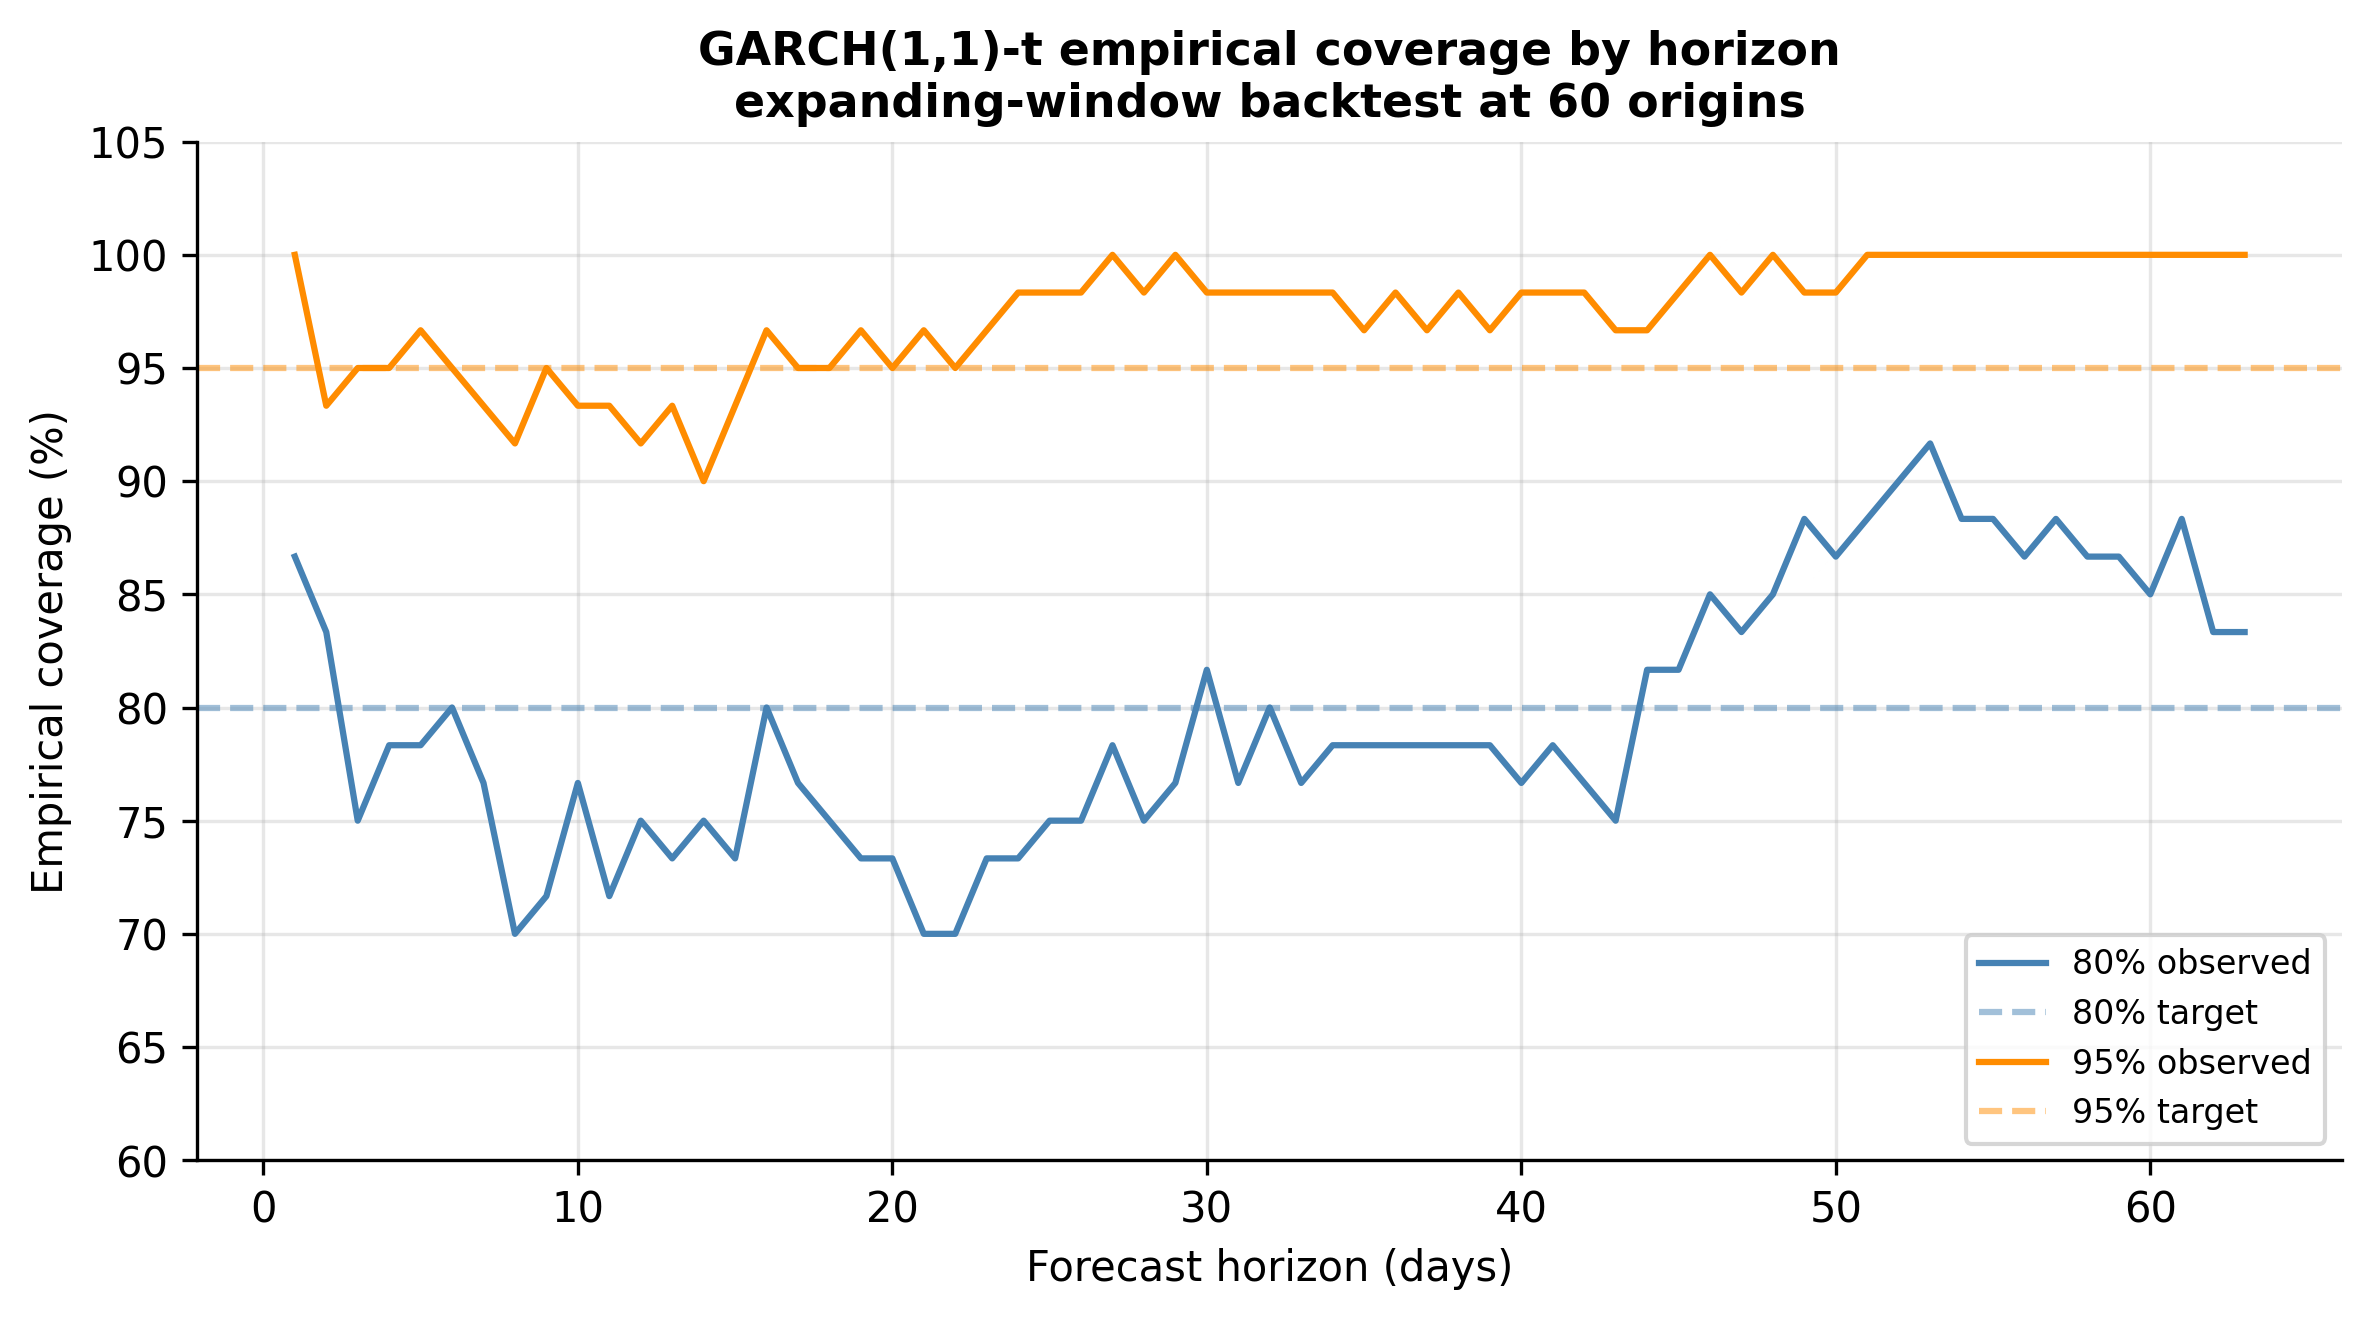
\includegraphics[width=0.75\textwidth]{garch_coverage.png}
\caption{Empirical coverage of GARCH(1,1)+$t$ prediction intervals at
the 80\,\% and 95\,\% levels as a function of forecast horizon, averaged
across the 60~origins.  Dashed lines show the nominal target rates.
Empirical coverage tracks the nominal rates within a small band at all
horizons evaluated.}
\label{fig:coverage_by_horizon}
\end{figure*}

Fig.~\ref{fig:fan_example} illustrates GARCH(1,1)+$t$ forecasts at six
origins spanning the breadth of price regimes in the backtest: calm
periods (Dec~2001, Dec~2018), moderate-volatility periods (May~2016,
May~2022), the 2011 rally (Mar~2011), and the 2024--2025 rally
(May~2025).  The figure makes visible the central operational feature of
the model: predictive-interval widths contract during calm regimes and
expand during turbulent ones, in proportion to conditional volatility at
each origin.  The 95\,\% band at Origin~5 (Dec~2001) is narrow,
reflecting the low-volatility conditions in late 2001; the corresponding
band at Origin~59 (May~2025) is roughly an order of magnitude wider in
absolute terms, reflecting the elevated volatility of the 2024--2025
rally.  All six realized paths fall within their 95\,\% prediction
intervals, with Origin~59 approaching the lower 80\,\% boundary but
remaining inside the 95\,\% band.

\begin{figure*}[t]
\centering
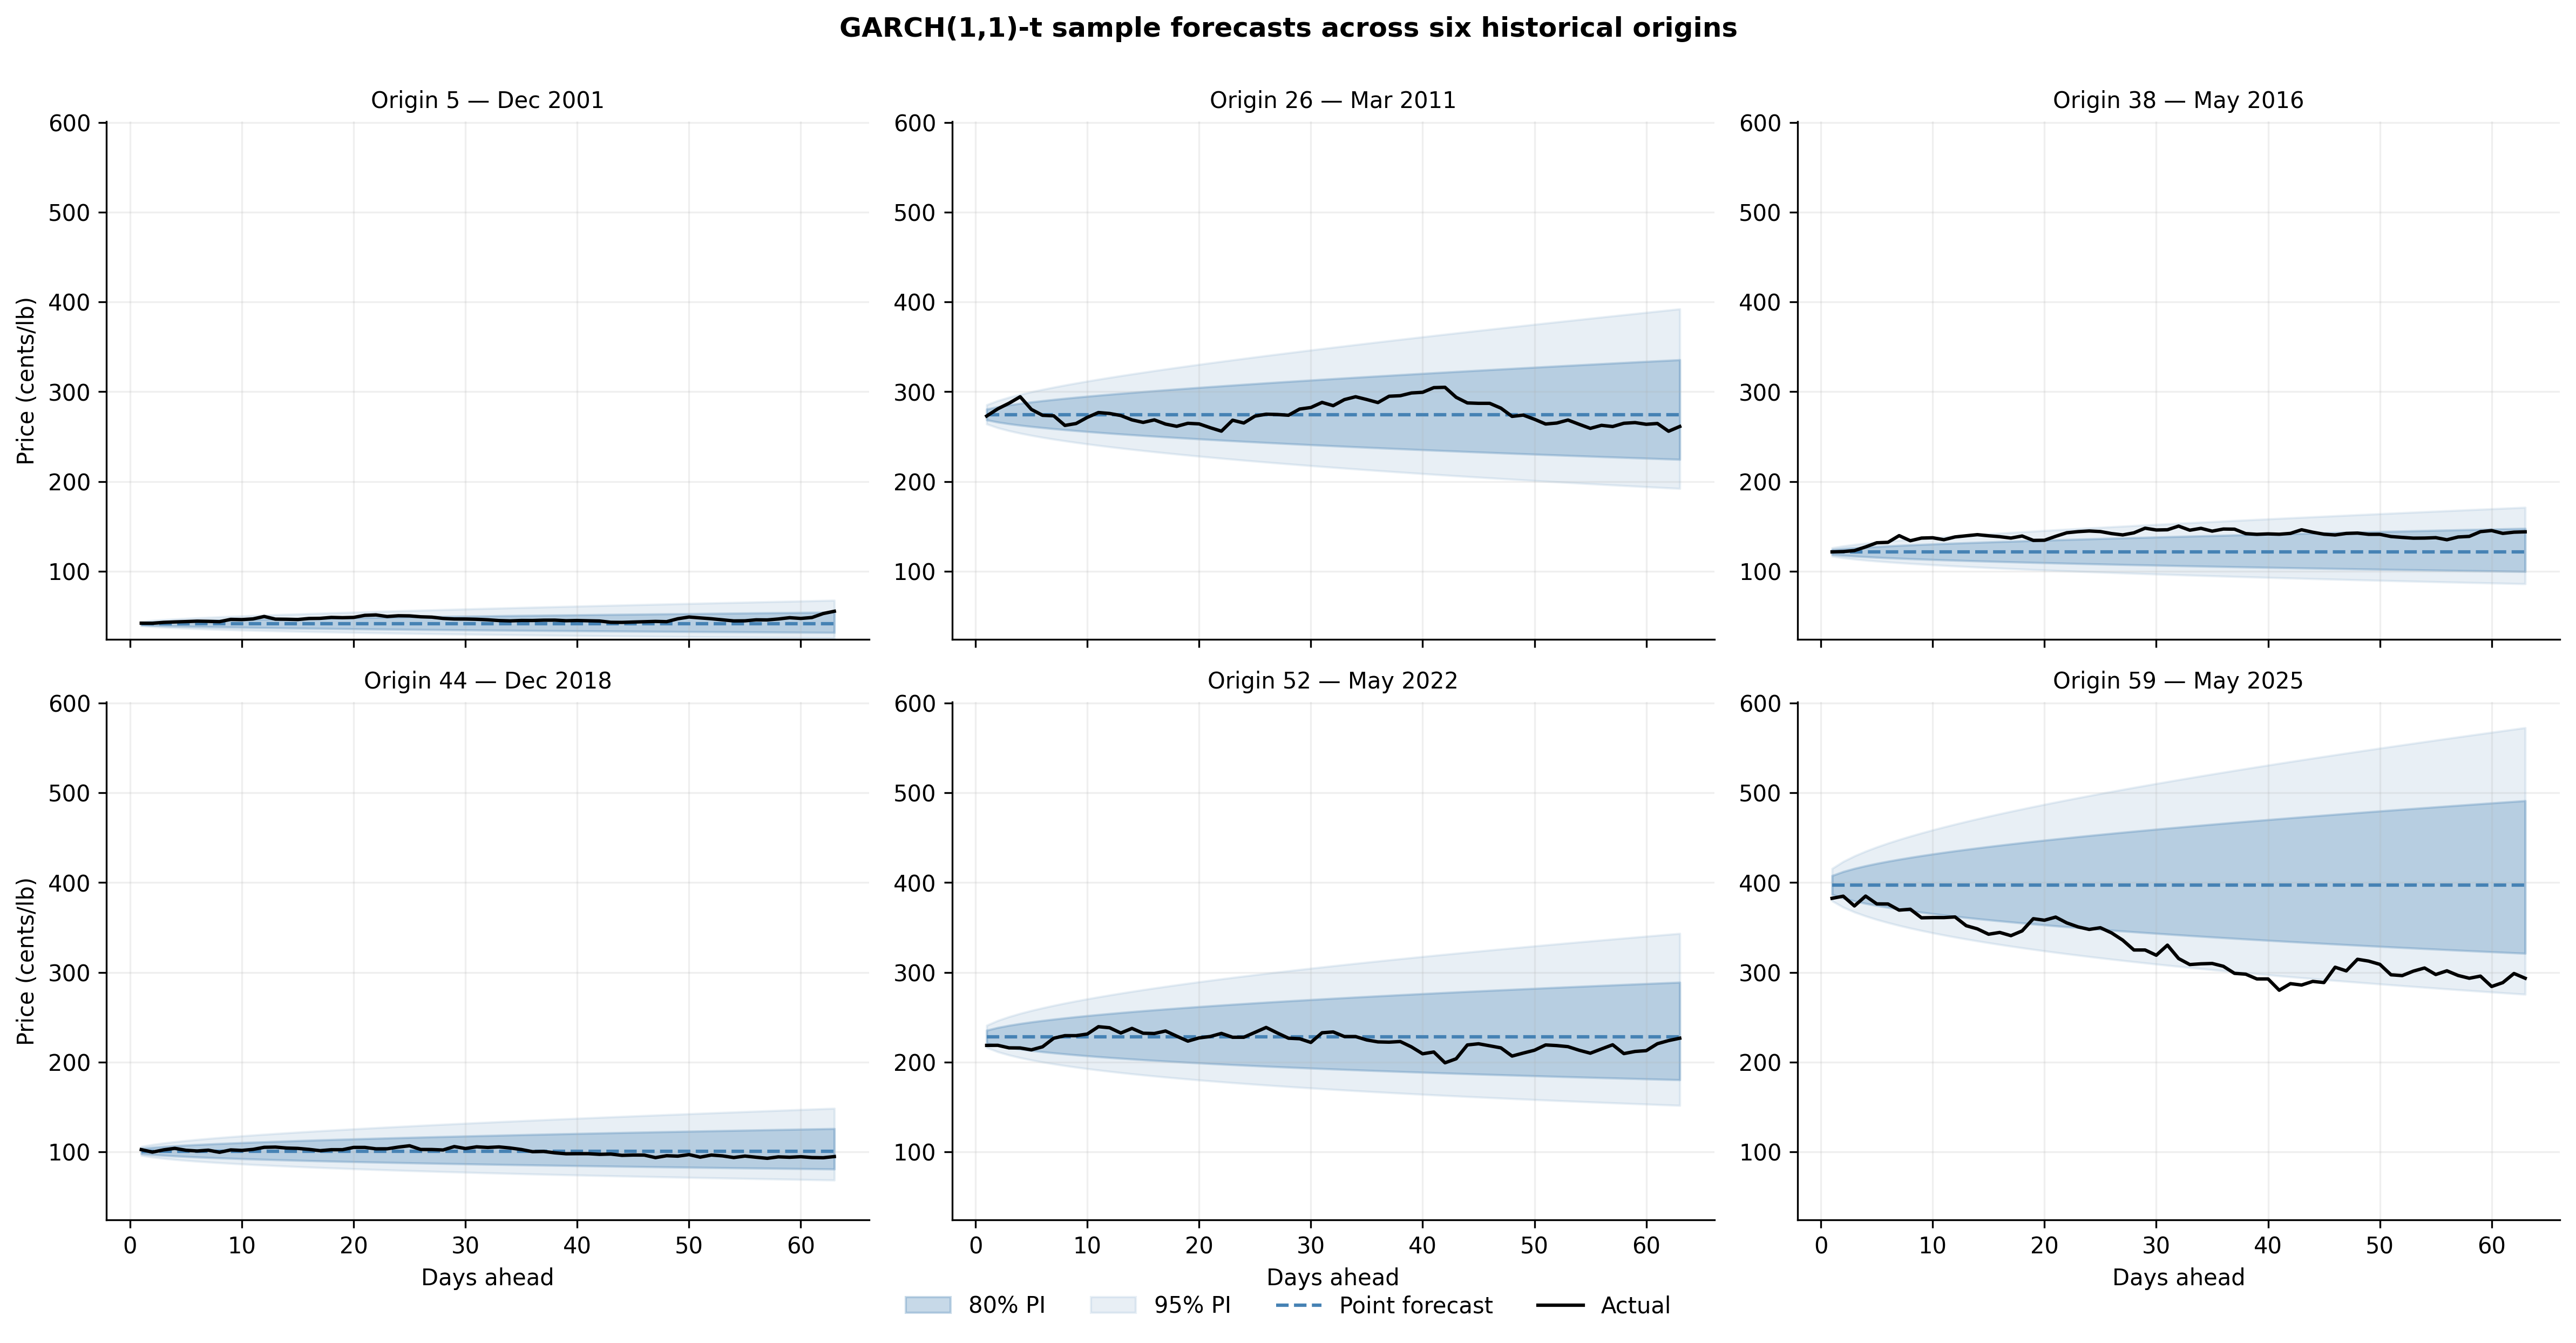
\includegraphics[width=0.95\textwidth]{garch_sample_forecasts.png}
\caption{GARCH(1,1)+$t$ sample forecasts at six historical origins from
the 60-origin backtest, spanning calm regimes (Dec~2001, Dec~2018),
moderate volatility (May~2016, May~2022), and major rallies (Mar~2011,
May~2025).  Each panel shows the point forecast (dashed), 80\,\% and
95\,\% prediction intervals (shaded), and the realized price path
(solid).  Interval widths adapt to local volatility: tight during calm
periods, wide during turbulent ones.}
\label{fig:fan_example}
\end{figure*}

\subsection{Discussion}
\label{sec:discussion}

\subsubsection{Why empirical coverage tracks nominal closely}
The pooled deviations in Table~\ref{tab:coverage_pooled} are small in
absolute terms---under 2.5~pp at every level evaluated---and mixed in
sign across the five nominal levels.  Two observations frame this
result.  First, the effective sample size is much smaller than the
$3{,}780$ raw forecast points: returns within a single 63-day forecast
trajectory are highly dependent, so the effective number of independent
trials is closer to the 60~origins.  Under that effective sample size,
the observed deviations sit within one standard error of nominal
calibration at every level---they are not statistically distinguishable
from perfect calibration.  Second, the mixed sign of the deviations
(under-coverage at the lower nominal levels, over-coverage at the
higher ones) is consistent with the empirical innovation distribution
being slightly more peaked but slightly thinner-tailed than the fitted
Student's~$t$.  No systematic bias is visible in the data.

\subsubsection{Regime adaptability and the limits of parametric tails}
Fig.~\ref{fig:fan_example} demonstrates the central operational strength
of GARCH(1,1)+$t$: predictive-interval widths scale with local
volatility, narrowing during calm periods and widening during turbulent
ones.  Parametric tail modeling has limits, however.  Even with the
heavier-tailed Student's~$t$ innovations, sufficiently extreme tail
events---those outside any reasonable parametric distribution---would
require non-parametric extensions (e.g.\ extreme value theory in the
tails), regime-switching variance dynamics, or sources of information
external to the price series itself (e.g.\ weather, inventory data) to
model directly.

\subsubsection{Limitations}
We model a single price series under a parametric GARCH(1,1) specification.
The literature contains numerous extensions---asymmetric variance dynamics
(GJR-GARCH, EGARCH), long-memory variants (FIGARCH), and stochastic
volatility models---that may further improve calibration; in tests on
equity indices these typically yield small marginal gains relative to a
well-specified GARCH(1,1)~\cite{hansenlunde2005}, but their performance on
commodities is less extensively documented.  Our backtest also fits all
parameters by maximum likelihood; Bayesian approaches that quantify
parameter uncertainty would yield wider predictive intervals at the cost
of additional computational complexity.

\subsection{Operational Implementation}
\label{sec:deployment}

The GARCH(1,1)+$t$ specification validated in Section~\ref{sec:results}
is implemented as an automated daily forecasting pipeline for 19~Coffee
Company.  Each trading day after market close, the pipeline appends the
latest settlement price to the historical series, refits the model on
all available history (matching the expanding-window design of the
calibration backtest), and produces an updated 63-day fan chart with
80\,\% and 95\,\% prediction intervals.  Price updates after the ICE
Report~293 archive cutoff are pulled from a real-time exchange data
feed; the historical training data underlying the backtest in
Section~\ref{sec:results} is unchanged.  Fig.~\ref{fig:live_forecast}
shows a representative output.  The continuously-refreshed fan
chart provides 19~Coffee with a current-state-aware estimate of plausible
3-month price trajectories, supporting procurement and budgeting
decisions on an ongoing basis rather than at a single fixed-date forecast.

\begin{figure*}[t]
\centering
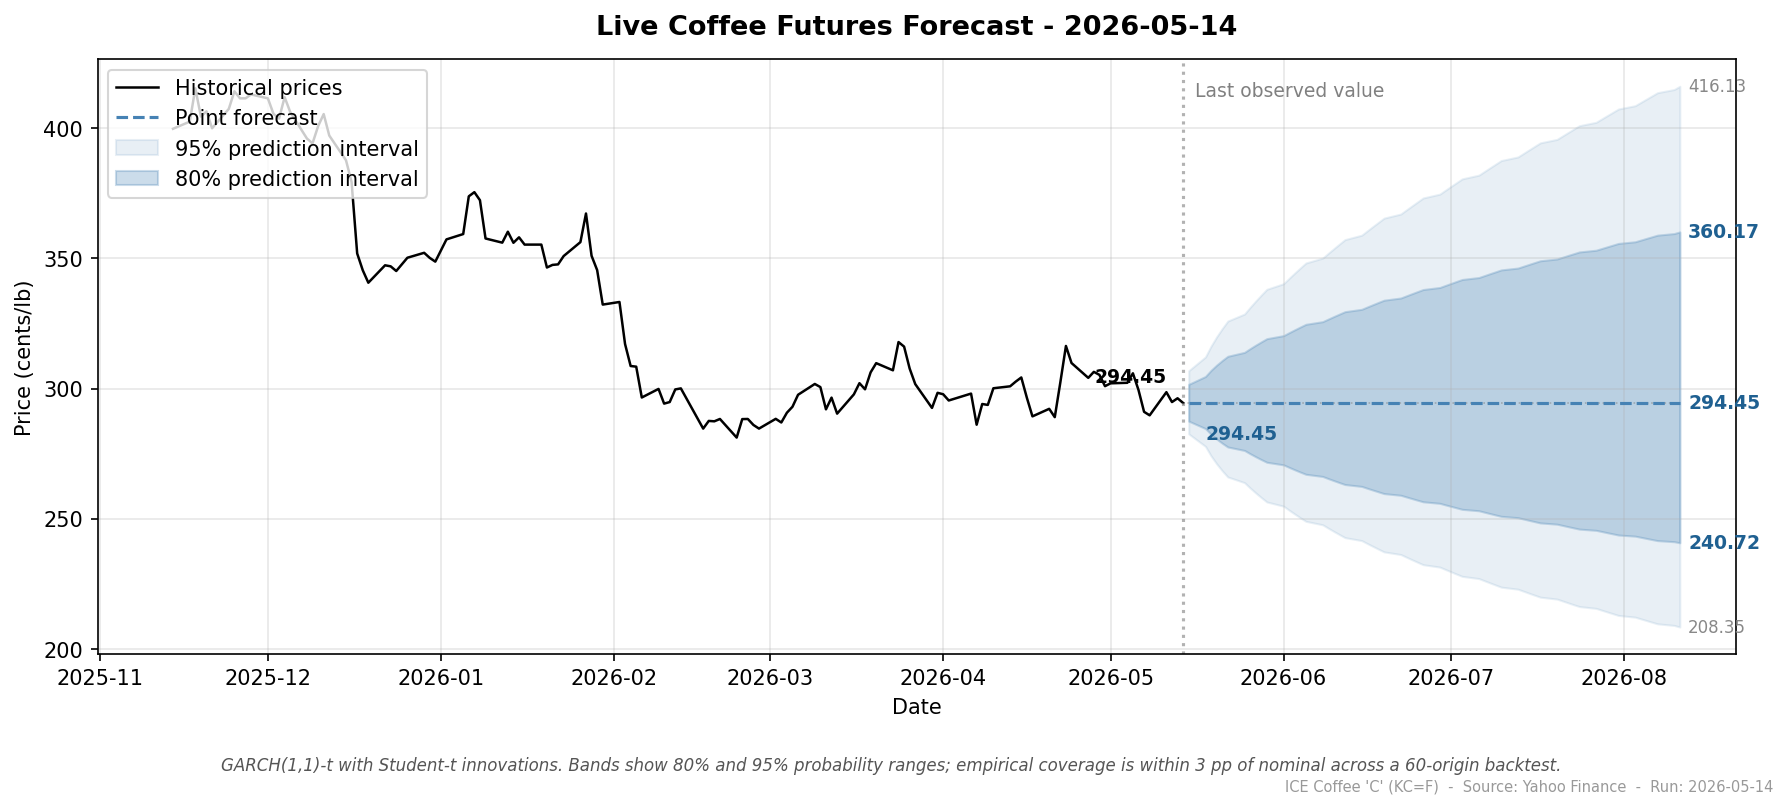
\includegraphics[width=0.75\textwidth]{latest_forecast.png}
\caption{Sample output of the operational forecasting pipeline,
generated on May~13,~2026.  Historical settlement prices (solid)
are followed by the 63-day point forecast (dashed) and the 80\,\% and
95\,\% prediction intervals (shaded).  The point forecast remains
approximately flat at the most recent settlement, consistent with the
near-zero conditional mean of returns; uncertainty grows with horizon
according to the model's conditional variance forecast.}
\label{fig:live_forecast}
\end{figure*}

% =============================================================
\section{Conclusion and Future Work}
% =============================================================
\label{sec:conclusion}

Section~I of this paper found that no point-forecast model in a
deliberately diverse ten-model suite could materially improve on a
random-walk-with-drift baseline for daily ICE Coffee~C futures prices,
with nine of ten models jointly indistinguishable from the best at
$\alpha=0.10$ on a Model Confidence Set test.  Section~II demonstrates
that this result is not evidence of an unstructured series.  When the
forecasting target is changed from a point estimate to a predictive
distribution, the persistent volatility clustering and fat-tailed
innovations in coffee returns become exploitable: a GARCH(1,1) model with
Student's~$t$ innovations, fit on expanding training windows and evaluated
at 60~origins, produces prediction intervals whose empirical coverage
tracks nominal coverage within a few percentage points at every level
evaluated, with interval widths that adapt to local volatility across
diverse historical regimes.

For 19~Coffee Company, this means the deliverable is not a price oracle
but an honest uncertainty band: at any given trading day, the GARCH-$t$
model produces an 80\,\% interval whose realized coverage tracks its
nominal rate closely, and which is meaningfully tighter during calm
volatility regimes and wider during turbulent ones.  Such an interval
supports concrete decisions---when to lock in a purchase, how much
budget reserve to maintain, when to escalate procurement
discussions---in ways that a point forecast cannot.

The methodological lesson generalizes beyond coffee: scoring a forecast
by MAE answers a different question from scoring it by interval coverage,
and the right scoring rule depends on the downstream decision the forecast
informs.  When decisions involve risk management, position sizing,
derivative pricing, or any task sensitive to the spread of possible
outcomes, density forecasts are strictly more informative and should be
evaluated as such.

Several extensions suggest themselves.  An out-of-sample comparison
against asymmetric GARCH variants and stochastic-volatility models would
clarify whether further calibration gains are available.  Multi-asset
joint modeling---in particular against the Brazilian Real and Arabica/Robusta
spreads---may exploit cross-market information unavailable to the
univariate GARCH framework.  Finally, augmenting the parametric tail
model with extreme-value methods would provide additional robustness
during extreme regimes.

% =============================================================
\section*{Acknowledgment}
% =============================================================

The authors thank Dr.~Jeffrey~P.~Wheeler of the Department of Mathematics,
University of Pittsburgh, for proposing this project and for ongoing guidance.

% =============================================================
\bibliographystyle{IEEEtran}
\bibliography{references}
% =============================================================

\end{document}
